\documentclass[12pt,]{article}
\usepackage{lmodern}
\usepackage{amssymb,amsmath}
\usepackage{ifxetex,ifluatex}
\usepackage{fixltx2e} % provides \textsubscript
\ifnum 0\ifxetex 1\fi\ifluatex 1\fi=0 % if pdftex
  \usepackage[T1]{fontenc}
  \usepackage[utf8]{inputenc}
\else % if luatex or xelatex
  \ifxetex
    \usepackage{mathspec}
  \else
    \usepackage{fontspec}
  \fi
  \defaultfontfeatures{Ligatures=TeX,Scale=MatchLowercase}
    \setmainfont[]{Arial}
\fi
% use upquote if available, for straight quotes in verbatim environments
\IfFileExists{upquote.sty}{\usepackage{upquote}}{}
% use microtype if available
\IfFileExists{microtype.sty}{%
\usepackage{microtype}
\UseMicrotypeSet[protrusion]{basicmath} % disable protrusion for tt fonts
}{}
\usepackage[margin=1in]{geometry}
\usepackage{hyperref}
\hypersetup{unicode=true,
            pdftitle={Artigo 1},
            pdfauthor={Thiago Mendes Rosa},
            pdfborder={0 0 0},
            breaklinks=true}
\urlstyle{same}  % don't use monospace font for urls
\usepackage{graphicx,grffile}
\makeatletter
\def\maxwidth{\ifdim\Gin@nat@width>\linewidth\linewidth\else\Gin@nat@width\fi}
\def\maxheight{\ifdim\Gin@nat@height>\textheight\textheight\else\Gin@nat@height\fi}
\makeatother
% Scale images if necessary, so that they will not overflow the page
% margins by default, and it is still possible to overwrite the defaults
% using explicit options in \includegraphics[width, height, ...]{}
\setkeys{Gin}{width=\maxwidth,height=\maxheight,keepaspectratio}
\IfFileExists{parskip.sty}{%
\usepackage{parskip}
}{% else
\setlength{\parindent}{0pt}
\setlength{\parskip}{6pt plus 2pt minus 1pt}
}
\setlength{\emergencystretch}{3em}  % prevent overfull lines
\providecommand{\tightlist}{%
  \setlength{\itemsep}{0pt}\setlength{\parskip}{0pt}}
\setcounter{secnumdepth}{5}
% Redefines (sub)paragraphs to behave more like sections
\ifx\paragraph\undefined\else
\let\oldparagraph\paragraph
\renewcommand{\paragraph}[1]{\oldparagraph{#1}\mbox{}}
\fi
\ifx\subparagraph\undefined\else
\let\oldsubparagraph\subparagraph
\renewcommand{\subparagraph}[1]{\oldsubparagraph{#1}\mbox{}}
\fi

%%% Use protect on footnotes to avoid problems with footnotes in titles
\let\rmarkdownfootnote\footnote%
\def\footnote{\protect\rmarkdownfootnote}

%%% Change title format to be more compact
\usepackage{titling}

% Create subtitle command for use in maketitle
\providecommand{\subtitle}[1]{
  \posttitle{
    \begin{center}\large#1\end{center}
    }
}

\setlength{\droptitle}{-2em}

  \title{Artigo 1}
    \pretitle{\vspace{\droptitle}\centering\huge}
  \posttitle{\par}
    \author{Thiago Mendes Rosa}
    \preauthor{\centering\large\emph}
  \postauthor{\par}
      \predate{\centering\large\emph}
  \postdate{\par}
    \date{2019-10-25}

\setlength\parindent{24pt}
\usepackage{indentfirst}
\usepackage{datetime}
\usepackage{setspace}
\onehalfspace
\usepackage{pdfpages}
\usepackage{floatrow}
\usepackage{amsmath}
\usepackage{morefloats}
\usepackage{pbox}
\usepackage{graphicx}
\usepackage{tikz}
\usepackage{booktabs}
\usepackage{tabularx}
\floatplacement{figure}{H}
\floatsetup[figure]{capposition=top}
\floatsetup[table]{capposition=top}
\usepackage[bf]{caption}
\captionsetup{justification=raggedright,singlelinecheck=false}
\usepackage{placeins}
\usepackage{rotating}
\usepackage[hyphenbreaks]{breakurl}
\usepackage{pdflscape}

\begin{document}
\maketitle

\hypertarget{abstract}{%
\section{Abstract}\label{abstract}}

We investigate the relationship between broadband internet and election
outcomes in Brazil for 2008, 2010 and 2012. Using a robust
identification strategy, a RDD aplied to the roll out of Backhaul
program, we explore jumps in internet velocity according to population
size. Results indicate no relationship between broadband and political
outcomes -- turnout, blank and null percentage votes and left parties
vote share. Our findings diverge from some results reported before,
suggesting that this relationship may differ in different contexts.

\hypertarget{introduction}{%
\section{Introduction}\label{introduction}}

The way how people get informed about politics has changed dramatically
over the years. If in XIX century press was the main source of
information, in the beginning of XX's radio took its place, surpassed by
television in the middle of the same century. Today, a new type of media
seems to be taking the lead: the internet.

Although the world wide web is a 25 years-old technology, broadband
connection is an even recent event. Internet velocity capable of
streaming videos became popular just in the XXI century. Social
networks, like You Tube, Facebook and Twitter are relatively infant
phenomenons, becoming popular globaly only in the late of 2000's. Mobile
broadband connections, thanks to 3G technology and massification of
smartphones, helped internet reach a greater number of users. New social
medias, like WhatsApp and Telegram are now everyday tools, with
popularity increasing in an exponential fashion, being important even
for business. A new wave, with 5G technology and the ``internet of
things'' is coming to continue the revolution begun in the past century,
with connections speed and quality increasing every day.

Thus, information dissemination gained range and speed, reaching more
people, almost instantaneously, nearly in any part of the world.
Geographic barriers were broken and the amount of information are vast.
Before these new possibilities, a question arises: how this new scenario
affects social interaction? Furthermore, how do people are doing
politics in this new environment? In particular, if people have tools to
be more informed, do they increase their participation in elections?
Could vote preferences change with introduction of this new technology?
Or, on contrary, have this new possibilities of entertainment deviate
people from political discussion? Is it possible that internet did not
change at all politics?

These questions are not easy to be answered for several reasons.
Availability of internet is not random and characteristics like income,
schooling and geographic conditions may determine if an internet service
provider will be accessible for individuals. Also, institutional and
political backgrounds may possible influence internet-political
relationship.

This is not a novel issue. Relationship between internet and politics
has been focus of study in severel fields, and this paper aims to
contribute with this literature, studying internet impacts on politics
in Brazil. Studying a single country gives us best tools to control
possible confounders, and using a robust identification strategy, we
take advantage of a specific rule for broadband roll out that creates an
instrument to deal with internet endogeneity, where number of
inhabitants determines the internet velocity of municipalities (the
backhaul program).

Results suggests that broadband internet are not related to political
outcome in Brazil. It seems that internet did not influnce turnout,
blank or null percentage votes and left parties vote share, in 2008,
2010 and 2012 elections, which covers national and local elections. The
office considered (president, mayor or deputies) did not make difference
in results. These finds are different from other results reported in the
literature, meaning that institutional background may play an important
role in political studies. Positive and negative relationship are
reported for Germany, Italy and United Kingdon (Falck \emph{et al.}
2014; Gavazza \emph{et al.} 2015; Campante \emph{et al.} 2017), all of
them with distinct political institutional background.

This paper is organized as follows: the first section presents the
theoretical framework linking internet to political outcomes, while the
next one reports the previous findings regarding its aplication. The
third section reviews the Brazilian political background, followed by
the section with empirical strategy, data bases and descriptives. The
fifth section presents our results, with a final discussion in the sixth
and last section.

\hypertarget{theoretical-framework}{%
\section{Theoretical framework}\label{theoretical-framework}}

There are some theories that try to explain why people vote (Downs 1957;
Riker \& Ordeshook 1968; Ferejohn \& Fiorina 1974; Uhlaner 1989; Aldrich
1993). One approach is to treat as a microeconomic problem in the
following way. In elections, individuals' problem is to choose the best
candidate(s) according to their preferences. But, there is an asymmetry
of information: there are many candidates (not considering uncontested
elections), and voters are not fully informed about their habilities.
Acquire information about them is costly, since they have to spend
resources to consume information (e.g.~from television, radio,
newspaper, internet or another people), that may include money and time.
Show up to cast the vote in the ballot also requires resources
(transportation and time). More accurate decision requires more
information, which demands more resources, i.e.~is more costly. So, it
can be viewed as a maximization problem from the microeconomics point of
view, which can be solved by equalizing marginal costs and benefits.
Benefits can be viewed as the policies the most preferred candidate will
conduct, a civil duty or being party of the democratic process.

This problem changes over time with entrance of new technologies. For
example, when radio, television and internet were not available, there
were fewer options to people get informed about candidates. Also, there
were available less leisure alternatives. With emergence of radio, then
television and, finally, internet, these costs and substitution effects
may have changed. A first natural question that someone could have is:
did these new technologies affect the decision of voters? For newspaper,
Gerber \emph{et al.} (2009), Gentzkow \emph{et al.} (2011) and Drago
\emph{et al.} (2014) report effects on elections participation.
According to Strömberg (2004) and Horacio \& Monteiro (2014), radio
affects people perception about politics, while DellaVigna \& Kaplan
(2007), Enikolopov \emph{et al.} (2011), Durante \& Knight (2012),
Gentzkow (2006) and Oberholzer-Gee \& Waldfogel (2009) shows the impact
of television (through news) on elections results.

How about the internet? Relationship between internet and politics has
been investigated since the end of 1990's (Bimber 1998). The effect on
information acquisition may be ambiguous depending on the hypothesis
used: if internet makes available new possibilities of entertainment,
people may substitute the time spent learning about politics with these
new type of leisure; on the other hand, if internet bring to people new
sources of politics information and channels of discussion, people may
be pushed toward politics. Finally, the cost and the time needed to find
candidates information or to find new possibilities of entertainment may
have changed relative prices. Once someone has access to internet, it is
possible to consume a variety of information with, in general, no
additional cost. The same is valid to leisure. A last possibility is
that the only thing substituted is the technology used to consume
information and leisure, making no difference at all in resources
allocation\footnote{If there is no, or little, consumption of politics
  information with an older technology, it might be the case that, even
  with a new technology, there is no preference for this type of
  information, resulting in no, or limited, shifting in its demand.}.

These changes may also take time to happen. Many types of media on
internet depends on broadband connection (like video streaming), only
available to the mass public in the beginning of the XXI century.
Moreover, all content we have today were not available with the launch
of the internet. The same was true for television, where the diversity
of programs and shows existing today took time to be developed and
aired. Emergency of new technologies and its spread also affects
relative prices both for information and leisure over time with this
development.

While newspaper, radio and TV content production are more restricted and
with barrier entries, internet have opened doors to virtually anyone
produce information and media, interact with people and organize groups
of common interest, everything at a low cost. Thus, it is likely to
exist a shift both in the demand and supply of information and
entertainment with internet arrival. It can potentially alter the manner
of how politics are made, since with internet politicians can reach more
people quickly and at low costs.

One situation this new scenario brings is the social media consumption
of fake news and its possible impact on elections. In the problem
treated here, misleading information may have a market that deviate
people from optimal choice (see Allcott \& Gentzkow 2017 for a
theoretical framework). Media capture by politicians put an additional
flavor to this discussion (Besley \& Prat 2006), where internet could
break other types of media control or enhance an existing control.

With this framework in mind, we analyse previous researches in the field
in order to collect results and identification strategies, pointing
resemblances and contrasts between them. Common outcomes between
internet and politics are voting turnout, election results, public
polices and politician's accountability.

\hypertarget{literature}{%
\section{Literature}\label{literature}}

Sources from where people consume information and leisure are not
exogenous. For example, if television or internet is expensive, only
people with enough income can have access. If this kind of people have
particular preferences regarding candidates, there is a bias if
relationship between internet and politic outcomes is treated as
unconditional. The same is valid for another characteristics, like race,
schooling, age or housing location.

Due to this endogeneity of internet supply and demand, geographical
characteristics (e.g landscape or rainfall) or previous
telecommunication infrastructure are common strategies used to
instrumentalize internet in order to link it to political outcomes.
Campante \emph{et al.} (2017) study the impact broadband diffusion on
political participation for municipalities of Italy between 1996 and
2013. Miner (2015) take similar path for Malaysia, Czernich (2012) and
Falck \emph{et al.} (2014) for Germany, Gavazza \emph{et al.} (2015) for
UK, Jaber (2013) for USA and Menezes (2015) for Brazil. With slightly
different approach, Lelkes \emph{et al.} (2017) explore variation in
state laws related to internet infrastructure to study influence of this
technology on polarization in USA, while Poy \& Schüller (2016) use
similar strategy to analyse broadband effects on turnout and vote share
in rural and sparse areas in Italy.

For Italy, Campante \emph{et al.} (2017) report a negative effect on
turnout in elections following high speed internet implantation (2008),
changing its direction for later elections (2013). An interesting result
reported in Italian case is that internet affected ideological groups
distinctly, according to vote share results, paving the way for
organization of new political groups, formed in online platforms. Poy \&
Schüller (2016) echoes these results, linking high speed internet
(ADSL2+) to increases in turnout in 2008 and 2013 Italian elections, as
well transitory increases in vote share of some parties (center-left and
right-fringe).

In Malaysian case, Miner (2015) reports important effects of internet in
2008 election results (vote share of opposition paties), but not in
turnout and limited effects in turnover. It is interesting to note that
the political background for the Malaysian case is different from the
Italian on, although the identification strategy is similar.

A negative effect of internet on turnout is reported by Falck \emph{et
al.} (2014) for Germany. The mechanism is related to an increase in
leisure consumption that crowds out television entertainment. The impact
reported is a heterogeneous one: west Germany was affect, while in east
Germany no effect was observed. Effects on vote shares were not
observed. On the other hand, Czernich (2012) found positive effects on
participation in German 2002-2005 election.

Gavazza \emph{et al.} (2015) report for UK negative effects of internet
on turnout in 2006-2010 elections, with stronger results for
less-educated and younger voters. Furthermore, incumbents seems to take
advantage, diminishing election competitiveness. Taking a step further,
the UK study suggests effects on public policies, lowering public
expenses and taxes in areas with higher internet access (with similar
heterogeneity effects reported for turnout).

In Brazilian case, Menezes (2015) shows that internet is associated with
increases in vote share of small candidates in 2010 elections, but no
relation with turnout nor with no candidates votes (blank votes). This
is an important result once the winner of last Brazilian presidential
election (2018) won with a very limited advertisement time on radio and
television in the first round.

For USA, results presented by Lelkes \emph{et al.} (2017) seems to bring
light to mechanisms underlying the effects of internet one politics
outcomes. States with less restrictive laws (and more likely to have
broadband coverage) induces people to be exposed to partisan information
and be more extreme in partisan preferences. This mechanism is
compatible with results presented in Jaber (2013), who reports a
positive impact on turnout, donations to political campaigns and
democrats vote share in 2008 presidential elections. In an early study,
with weaker identification strategy, Tolbert \& McNeal (2003) suggests
that, in 1996 and 2000 presidential election, individuals with internet
and online elections news are more likely to vote.

It is important to note that countries have distinct political regimes,
which could potentially affect results reported. Minard \& Landriault
(2015) bring this to discussion analysing how maturity of democracy
regimes in Asia responds to internet availability. Immature regimes
seems to be more affect by internet than solid democracies according to
2006 cross-country analysis. Hence, this cross country variation
suggests that there are institutional factors playing action on
internet-politics relationship, which puts caution to external validity
of results.

To sum up, it is clear that we have different results for different
countries (even inside the same country), with possible changing effects
over the time. Also, the majority of studies are concentrated in 2000
decade elections, take advantage of the begging of the internet. Few
studies report results for elections held in 2010 decade, when
smartphone revolution and social media gained strength. Even more, there
are no studies about the offects of mobile broadband and smartphones on
elections.

In this paper we will address just fixed line broadband roll out,
studying the Brazilian case, one of the largest democracies in the
world. Unfortunatly, mobile broadband techonology roll out (3G and 4G)
will not be investigated, since information at municipality level is not
available. As pointed before, peculiarities of each country seems to be
determinant for results, which demands closer analysis of the political
system in order to compare our results with those presented before.

\hypertarget{brazils-background}{%
\section{Brazil's background}\label{brazils-background}}

Brazil is a federative republic, with three layers of government:
central (or federal), states and municipalities. It is a young
presidential democracy, with bicameral legislative system (Chamber of
Deputies and Senate), holding election every four years. President is
elected by direct vote since 1989 in national elections, being elected
together with national congress, state governors and state assemblies
(1994 onward). Local elections, for municipal mayors and local
legislatives are also held every four years, since 1996\footnote{Brazilian
  dictatorship ended in 1985, with general election in 1986, except for
  president (elected indirectly in the previous year). Before 1985, all
  other elections (except for president) had direct vote, but under
  military rules. In 1988, a new constitution was promulgated and in
  1989 the president was elected by direct vote again, after 29 years.
  In 1990, there were elections for state governors, state assemblies
  and national congress. In 1992, municipal mayors and local assembly
  members were elected. By 1994 onward, national elections (president,
  state governors, state assembly and national congress) happens every
  four year, while local elections (municipal mayor and municipal
  assembly) happens every four years, since 1996. Thus, Brazil have
  elections every two years since 1994.}.

In Brazil, voting is mandatory to literate citizens aged 18 to 69. For
people aged 16 to 17 and over 70 voting is optional. Voters absent in
election must justify or pay a small fine. If they fail to justify three
consecutive pools, some rights are lost (issue or renew passports and
national identification, ineligible for public education, public service
and some government social programs). This set raises the question if
this rule changes incentives to acquire information about politicians.

An important aspect of Brazilian suffrage regards campaign
advertisement. There are national, free of charges and mandatory
programs during campaign time, booth aired daily in radio and
television, broadcasting the same content in all regions of the country.
There is a fixed amount of time for electoral advertisement in these
channels, 2/3 distributed according to current party presence in
legislatures and 1/3 among candidates, and only this time is allowed to
be used in these channels. Ads on newspaper are also restricted, even
though being a less important media compared to TV and radio. Internet
is exception, where candidates can use, almost freely to reach voters,
since 2009, except for anonymously or paid advertisement (which includes
social medias like Twitter, Facebook and You Tube).

According to Downs (1957), low probability to be pivotal in elections
explain the ``rational ignorance'' of voters and low preference to turn
out. On the other hand, mandatory vote could change this incentives,
making people more inclined to vote (Lijphart 1997). Leon \emph{et al.}
(2014) finds that, for Brazilian case, mandatory voting seems not change
people incentivesb to be more informed in voting decision. It seems the
case that providing more information about candidates (Banerjee \emph{et
al.} 2011), hence lowering the costs for collect information, is more
effective than compulsory voting system.

Following Fujiwara \emph{et al.} (2016), we try to considering possible
persistent habits on voting pattern, incorporating raining information
in election days in each municipality.

\hypertarget{empirical-strategy-and-data-bases}{%
\section{Empirical strategy and data
bases}\label{empirical-strategy-and-data-bases}}

\hypertarget{communication-usage}{%
\subsection{Communication usage}\label{communication-usage}}

As a glimpse of brazilian communication consumption, Figure \ref{fig:0}
presents internet and cell phone usage from 2008 to 2017.

\begin{figure}
\centering
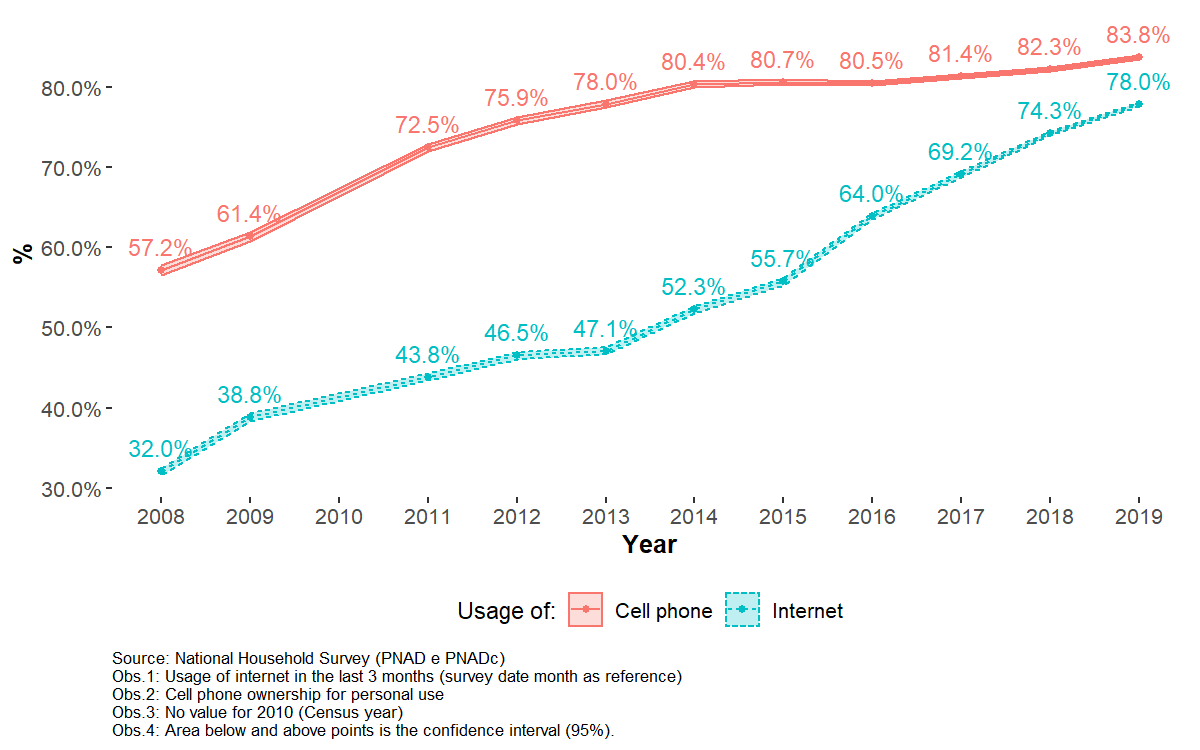
\includegraphics{artigo1_files/figure-latex/internet_usage-1.png}
\caption{Internet and cell phone usage in Brazil, \% of 16+ year-old
population, 2008-2009 and 2011:2017 \label{fig:0}}
\end{figure}

In 2008, 30\% of Brazilians (16 years-old or above, i.e.~population in
vote age) declared to have used internet at least once in the last three
months (September as reference), while almost 60\% declared cell phone
ownership for personal usage. In order to increase these figures, the
government carried out a national plan in the beggining of 2008. In
2011, these figures rose to 44\% and 73\%, respectively, indicating an
increasing communication market in Brazil. Even in 2017, there is room
remaining for internet and cell phone expansion in Brazil.

Hence, this expressive change in communication consumption may have
changed how Brazilians face politics, possibily increasing opportunities
for information acquisition and social interaction about this matter.
Or, on the other hand, widening leisure alternatives.

\hypertarget{backhaul-program-national-broadband-plan}{%
\subsection{Backhaul Program (National Broadband
Plan)}\label{backhaul-program-national-broadband-plan}}

In Appril 2008, the presidential Decree 6,424 changed the former
National Plan of Goals for Public Switched Telephone (PST) Network
Universalization, adding broandband infrastructure as mandatory (in
exhange of the PST obligation). The infrastruture reefered in the Decree
was the Backhaul, a requirement for internet implementation in the
country. Backhauls are necessary in order to connect them to the
Telephone Companies' Backbones. The plan put as target that, at least,
40\% of municipalities sould have the necessary infrastructure by the
end of 2008, 80\% by the end of 2009 and 100\% by the end of 2010. Also,
minimal internet velocities were set, increasing with population size
(Table \ref{tab:program_backhauk}).

\begin{table}[!h]

\caption{\label{tab:program_backhauk}Backhaul Plan}
\centering
\begin{tabular}{lrrr}
\toprule
Population Size & N\# municipalities & \% & Velocity (Mbps)\\
\midrule
Up to 20,000 & 3,077 & 90 & 8\\
From 20,001 to 40,000 & 268 & 8 & 16\\
From 40,001 to 60,000 & 63 & 2 & 32\\
Above 60,001 & 31 & 1 & 64\\
Total & 3,439 & 100 & NA\\
\bottomrule
\multicolumn{4}{l}{\textsuperscript{1} Source: Anatel, 2010.}\\
\end{tabular}
\end{table}

According to the Natiaonal Agency of Telecommunication (Anatel) (Anatel
2010), the majority of municipalities to be covered by Backhaul program
were up to 20,0000 inhabitants, which is more than half of total
municipalities of Brazil\footnote{Today, Brazil has 5,570
  municipalities. By the time when the program was created, six
  municipalities did not exist.}. The minimal required velocity (8 Mbps)
guarantee improvement in navegation quality, allowing, for example,
streaming (music and videos).

Out of 5,570 municipalities, by 2015, only 85 remained uncovered (Table
\ref{tab:desc_back}) and 2,125 (38\%) already had broadband
infrastructure before the program, mainly larger cities. We note that
the program focused on small cities, with average population under
15,000.

\begin{table}[!h]

\caption{\label{tab:desc_back}Backhaul deployment by year}
\centering
\begin{tabular}{lrrr}
\toprule
Situation & \# Munic & Avg Velocity & Avg Pop.\\
\midrule
Covered & 3,360 & 11 & 14,403\\
Covered before & 2,125 & NaN & 67,151\\
Uncovered & 85 & NaN & 35,372\\
Total & 5,570 & 11 & 34,072\\
\bottomrule
\multicolumn{4}{l}{\textsuperscript{1} Municipalities by backhaul status}\\
\end{tabular}
\end{table}

According to program schedule, 100\% of Brazlis' municipalities should
has backhaul infrastructure in 2010. However, by this year 72\% of the
goal was achieved. Table \ref{tab:backhaul_implementation} presents the
roll out of the program by year.

\begin{table}[!h]

\caption{\label{tab:backhaul_implementation}Backhaul deployment by year}
\centering
\begin{tabular}{lrrr}
\toprule
Backhaul year & \# Munic & Avg. Velocity & Avg Pop.\\
\midrule
2008 & 1,384 & 13 & 16,911\\
2009 & 1,388 & 10 & 13,340\\
2010 & 495 & 9 & 9,026\\
2011 & 27 & 2 & 12,134\\
2012 & 7 & 14 & 25,531\\
\addlinespace
2013 & 41 & 4 & 20,238\\
2014 & 17 & NaN & 38,490\\
2015 & 1 & NaN & 13,293\\
Total & 3,360 & 11 & 14,403\\
\bottomrule
\multicolumn{4}{l}{\textsuperscript{1} Source: Anatel.}\\
\multicolumn{4}{l}{\textsuperscript{2} Obs.: No velocity information for 2014 and 2015.}\\
\end{tabular}
\end{table}

The main point of our identification strategy rests on the velocity
descontinuity, which is futher analysed in Figures \ref{fig:1} to
\ref{fig:1.5}, by region, since Brazil is a continental country with
important regional inequalities. North and Northeast regions are poorer,
while South and Southeast are richer\footnote{For example, the state of
  São Paulo was responsible for almost 1/3 of Brazilian GDP in 2017. Per
  capita household income of the richest state (Federal District) was
  3.84 times greater than the poorest (Alagoas), according to 2014
  National Household Survey (IBGE/PNAD). Brazilian Gini index for the
  same year was 0.517.}, making a commoon practice disaggregated
analysis in Brazil.

\begin{figure}
\centering
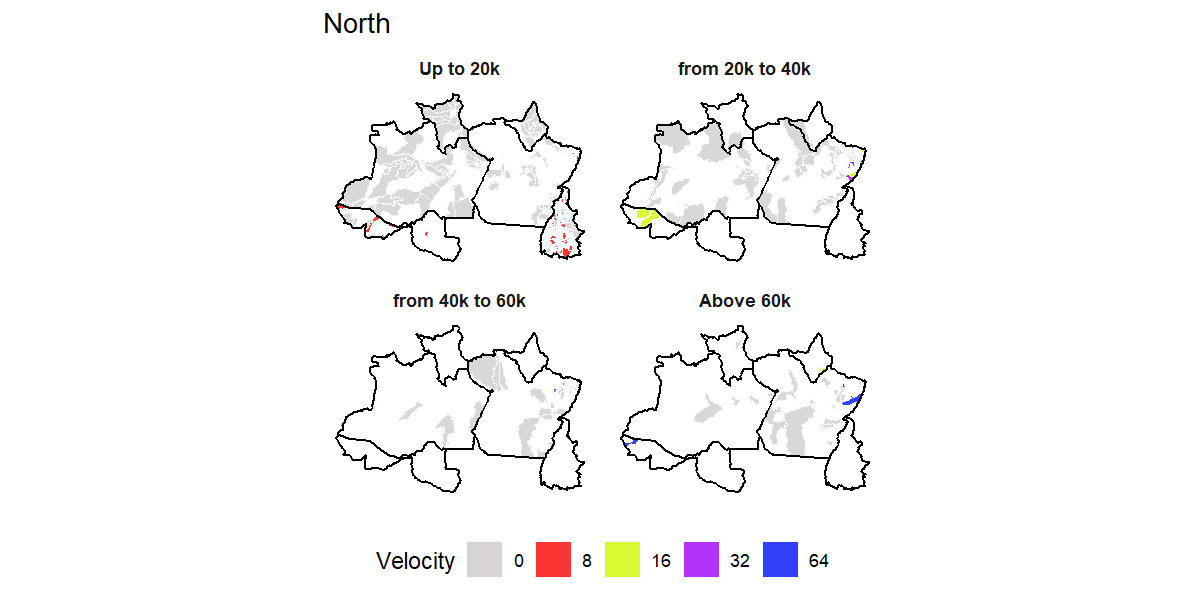
\includegraphics{artigo1_files/figure-latex/mapa-1.png}
\caption{Internet velocity in backhaul program by municipality
population, North region \label{fig:1}}
\end{figure}

\begin{figure}
\centering
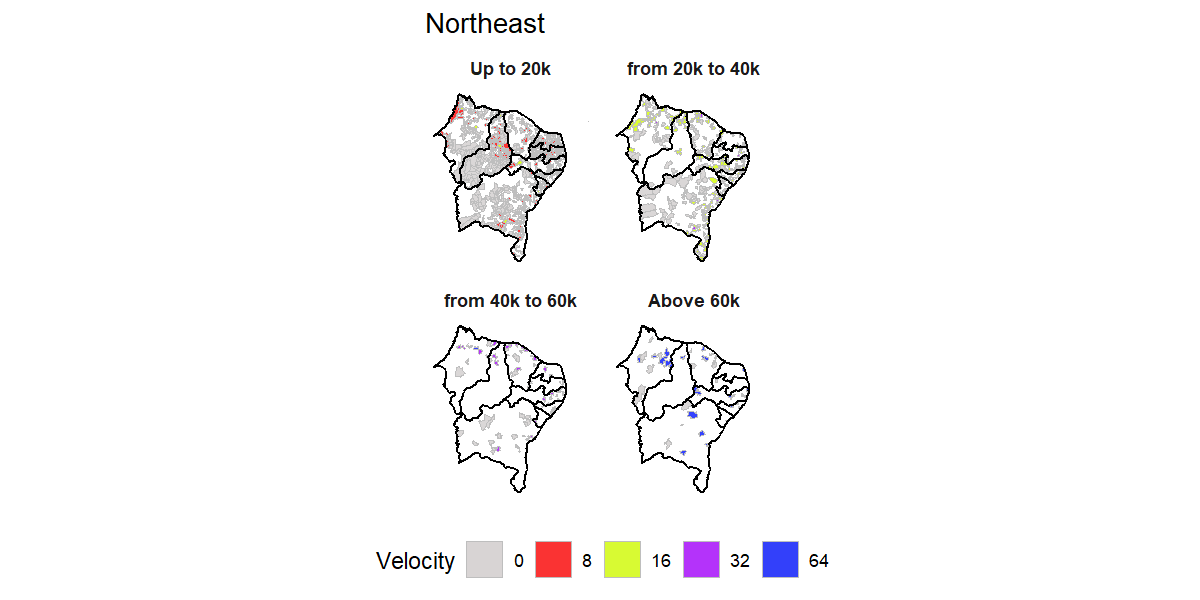
\includegraphics{artigo1_files/figure-latex/mapa2-1.png}
\caption{Internet velocity in backhaul program by municipality
population, Northeast region \label{fig:1.2}}
\end{figure}

\begin{figure}
\centering
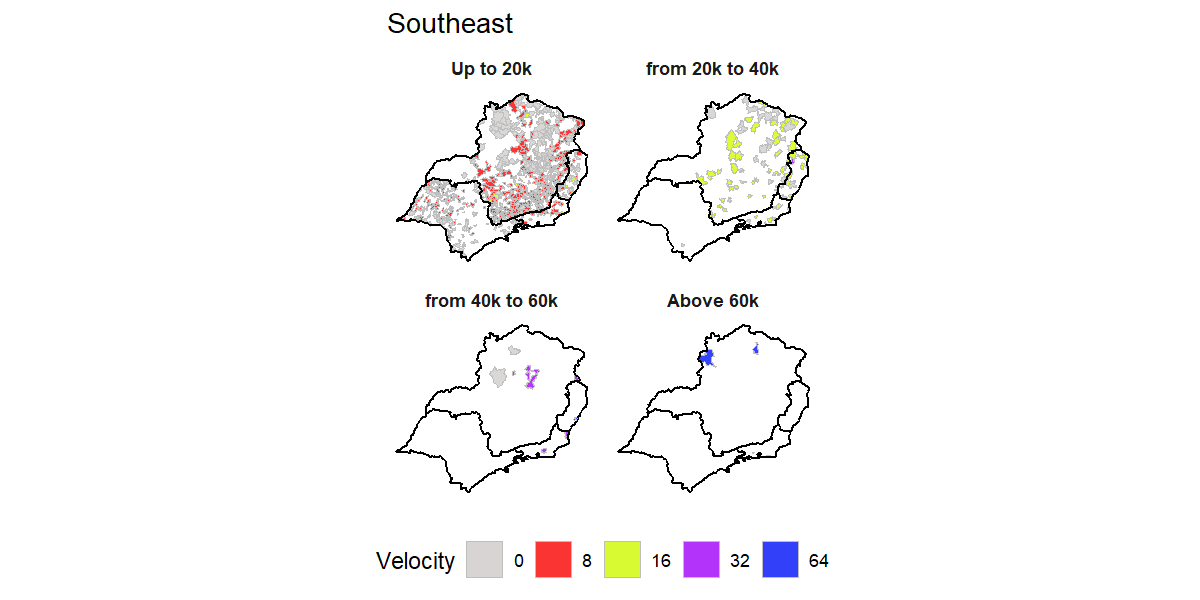
\includegraphics{artigo1_files/figure-latex/mapa3-1.png}
\caption{Internet velocity in backhaul program by municipality
population, Southeast region \label{fig:1.3}}
\end{figure}

\begin{figure}
\centering
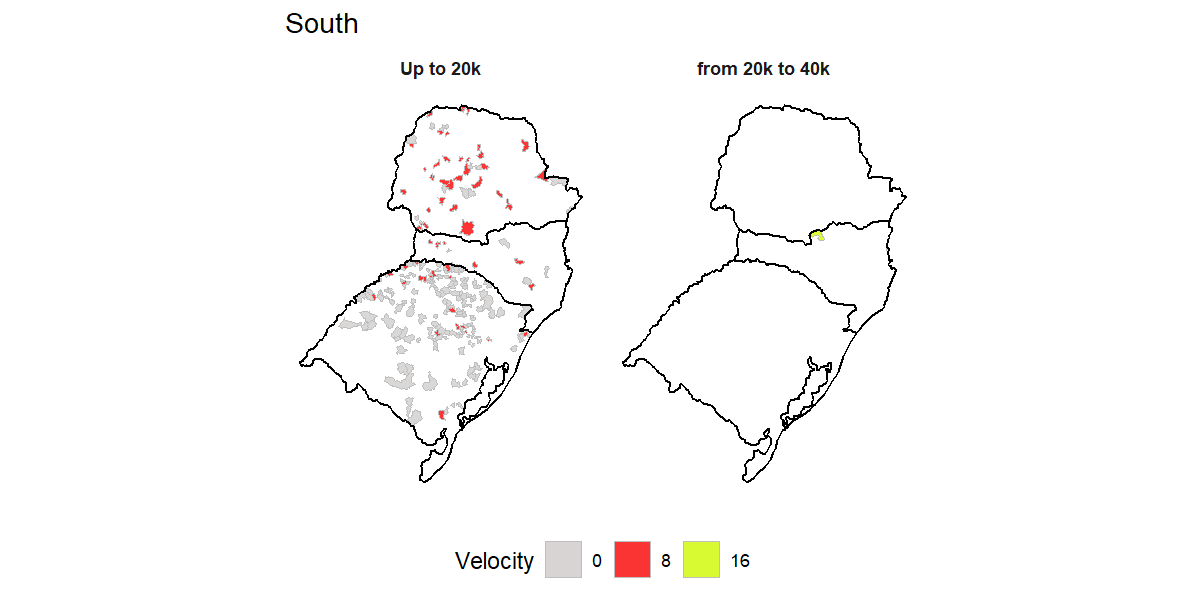
\includegraphics{artigo1_files/figure-latex/mapa4-1.png}
\caption{Internet velocity in backhaul program by municipality
population, South region \label{fig:1.4}}
\end{figure}

\begin{figure}
\centering
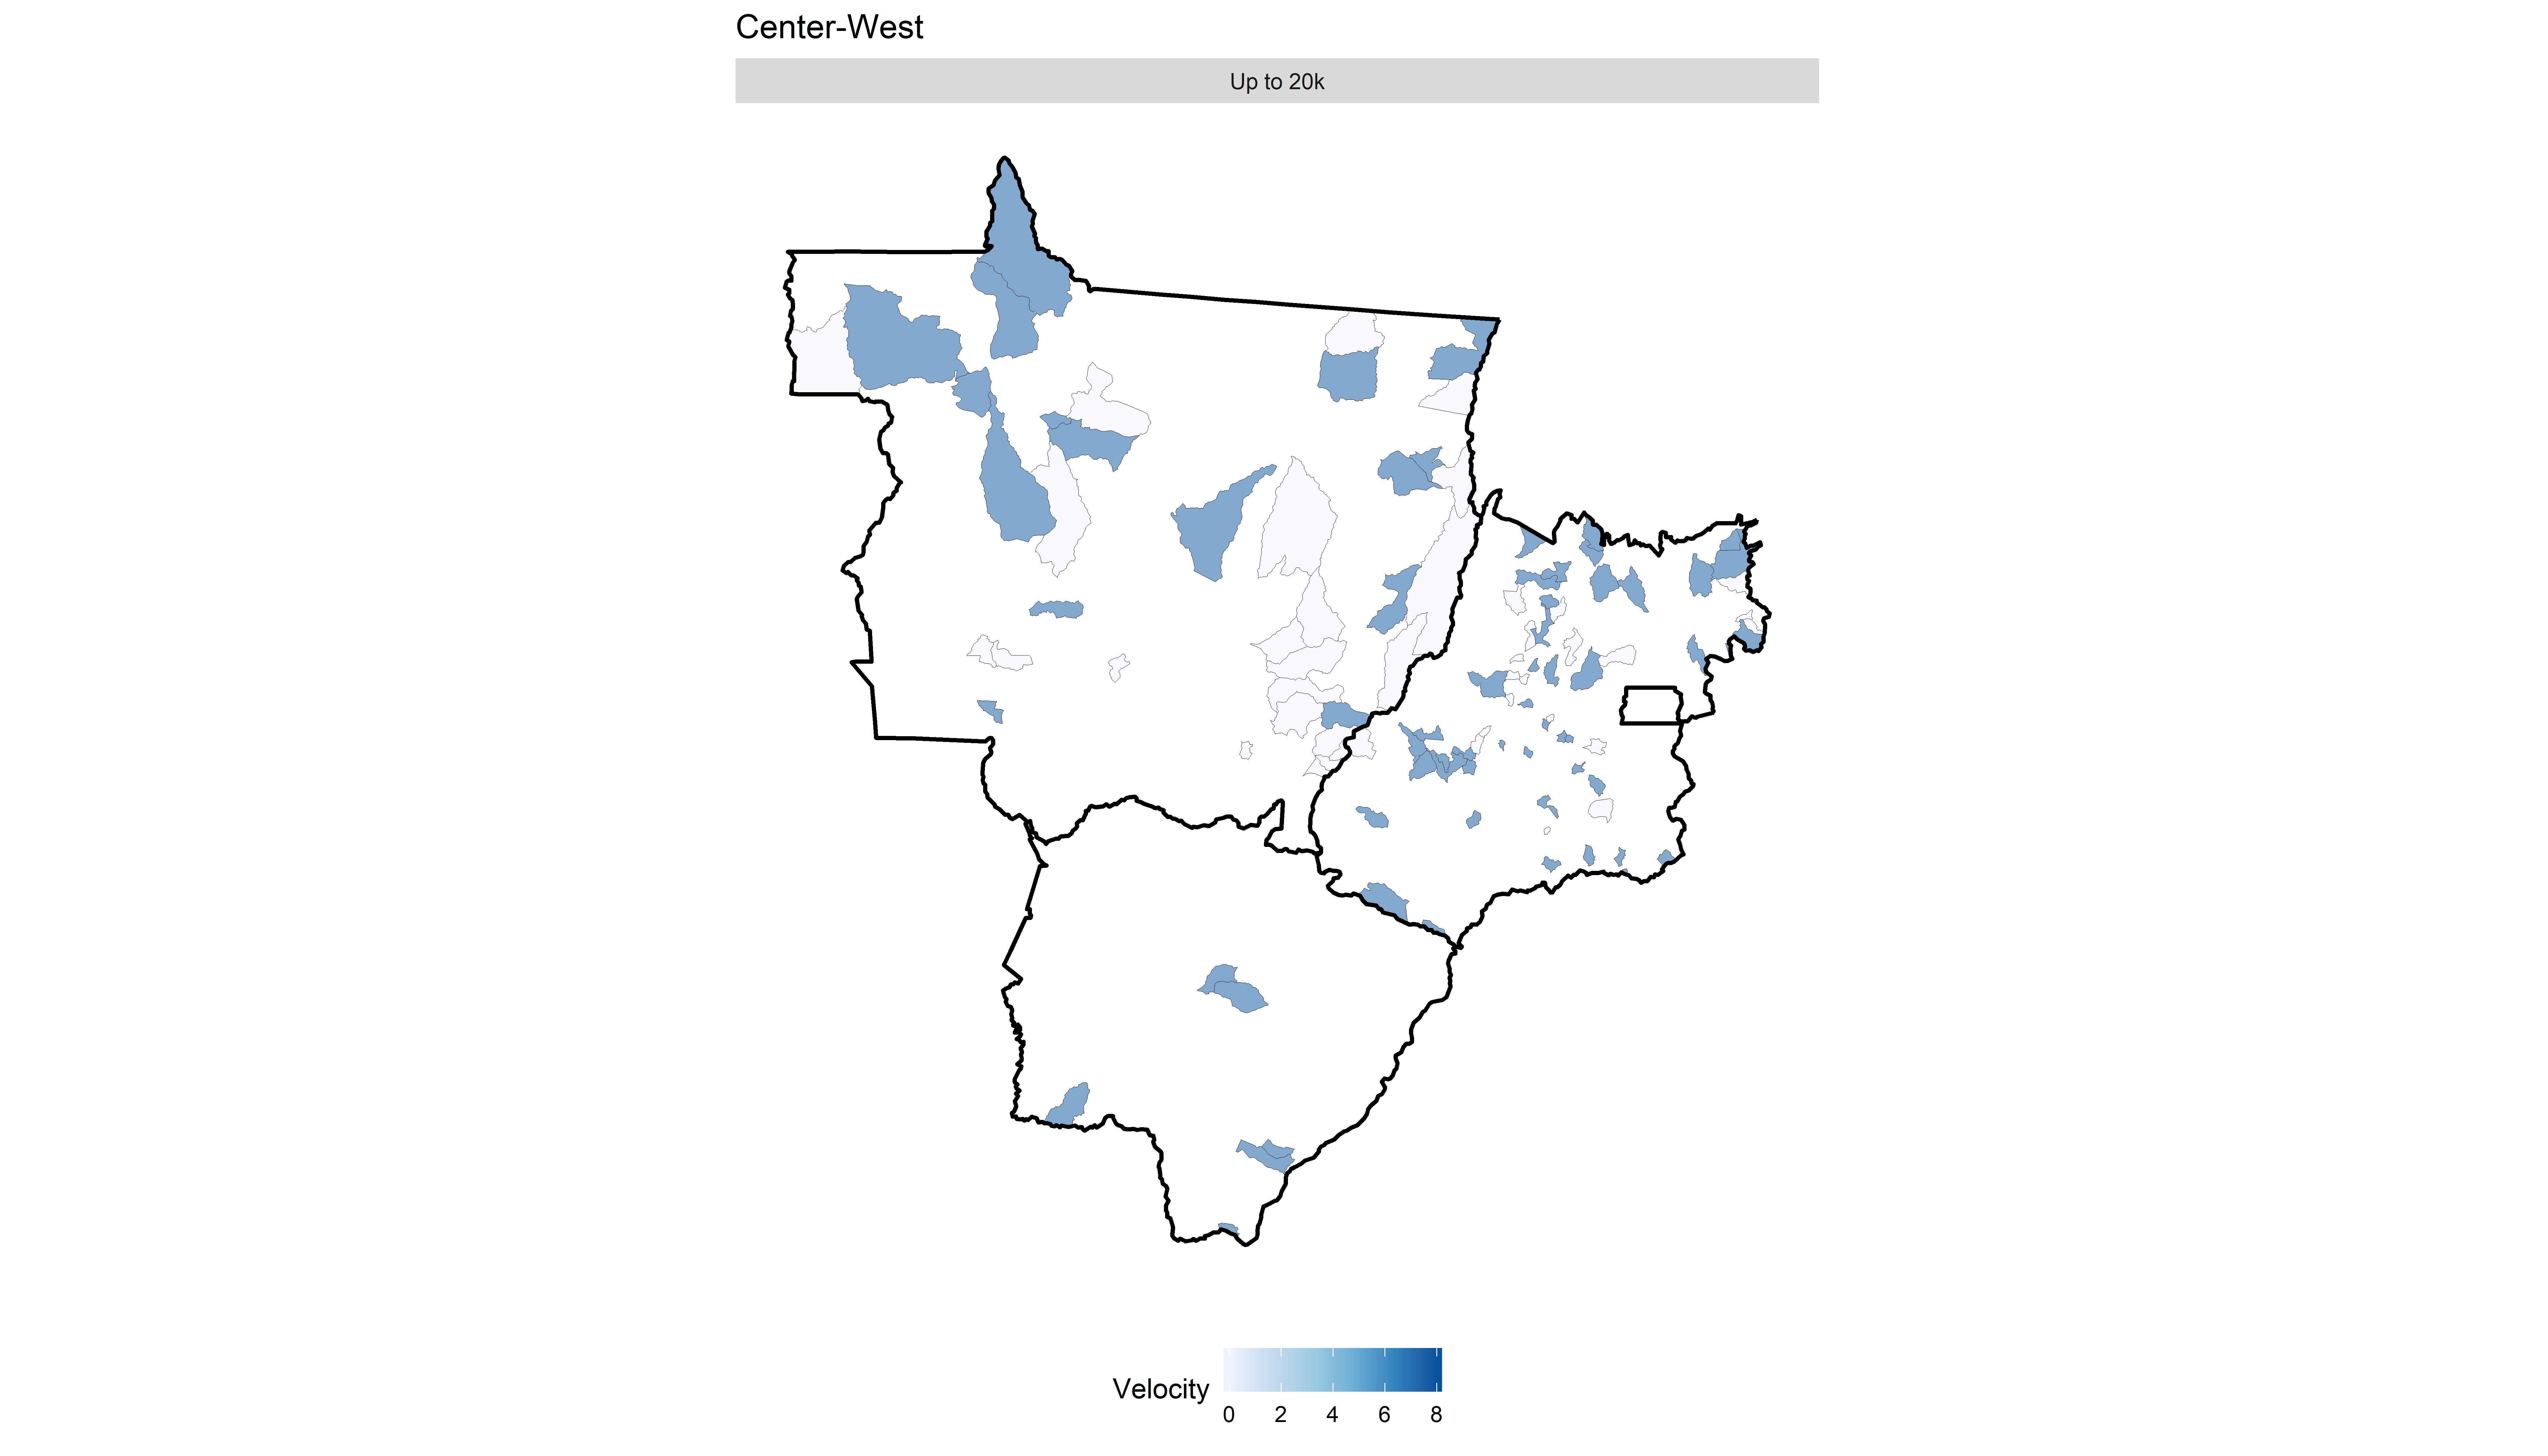
\includegraphics{artigo1_files/figure-latex/mapa5-1.png}
\caption{Internet velocity in backhaul program by municipality
population, Center-West region \label{fig:1.5}}
\end{figure}

\begin{figure}
\centering
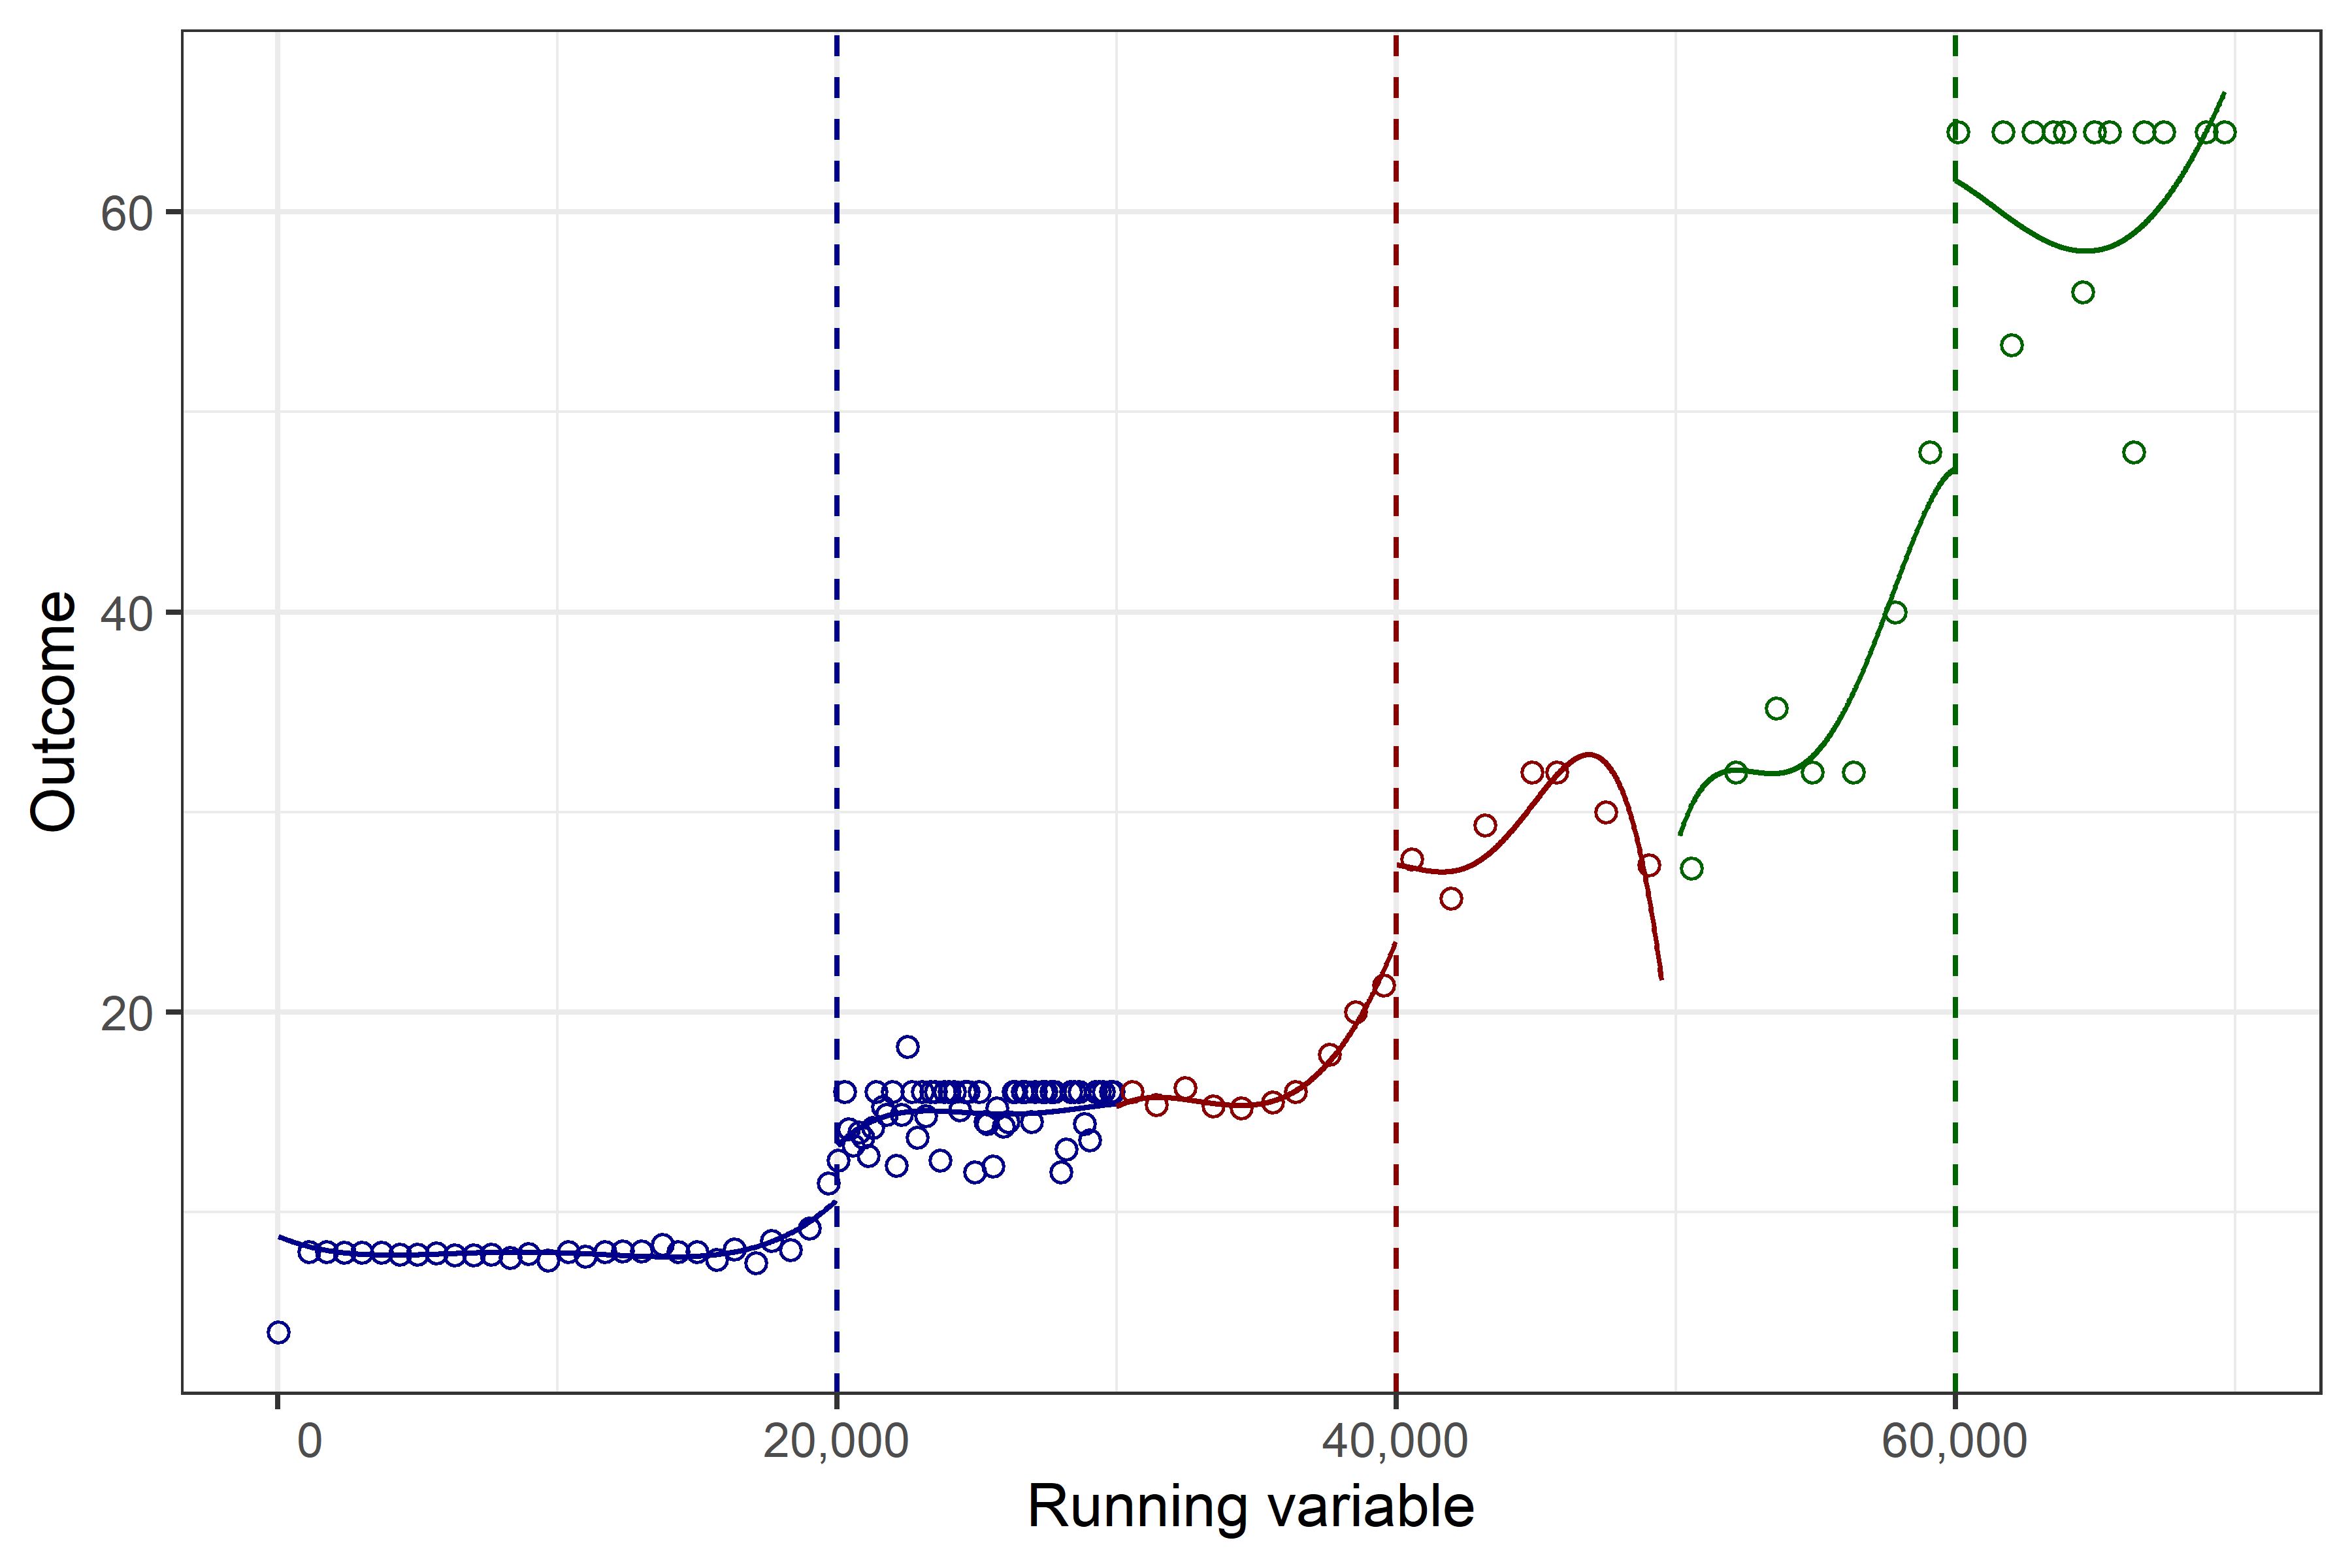
\includegraphics{artigo1_files/figure-latex/descontinuity-1.png}
\caption{Descontinuity in Backhaul program velocity by population
cut-offs: 20,000; 40,000; 60,000 \label{fig:2}}
\end{figure}

Figure \ref{fig:2} shows a clear jump in velocity cut-offs for the
entire period. The jump around cut-offs are clear, where municipalities
just below the population size estabilished in the program face lower
internet velocities. The first cut-off must be preferable due to sample
size, as well as pooled weighted estimations, which will also be
presented.

\hypertarget{descriptive-statistics}{%
\subsection{Descriptive statistics}\label{descriptive-statistics}}

Despite these clear descontinuities, a set of covariates were collected,
in order to control for any further confounder that might remain. Lack
of information at municipal level is one of the weakness in Brazilian
researchs at this territory level. Census occurs only every ten years,
remaining only few administrative data in the between years, some of
them with low quality (mainly for small cities). Even tough, considering
that this is the only source of the main socioeconomic variables, we use
information from the last two censuses (2000 and 2010), organized by
Brazilian Institute of Statistics and Geography (IBGE). Also from IBGE,
we collect total population estimates and GDP. Considering that direct
cash transfers are important in Brazil, we collect data from the two
major programs: Bolsa Família (PBF) and Benefício de Prestação
Continuada for elderies (BPC), booth organized by Ministry of
Citizenshipt\footnote{PBF is one of the biggest conditional cash
  transfer program in the world. The target are families under the
  extreme poverty and poverty lines (in 2019, families earning up to R\$
  89 by person, or U\$ 21, by month are considered extremely poor, while
  families above that amount and up to R\$ 178, or U\$ 40, are
  considered poor), focused one children. As counter part, school
  attendance and vaccination are required. PBF reachs almost 14 million
  families in Brazil in 2019. On the other hand, BPC is a program for
  elderly and handicapped. The poor population in this profile (people
  with or over 65 years and all handicapped) are eligible for a minimum
  wage paycheck.}. In additon, we collect the mass of wages (formal
labour market) from RAIS data base, organized by Ministry of
Economy\footnote{In Brazil, every formal company have to fill the Annual
  Relation of Social Information (RAIS), with the profile of all workers
  they had in the calendar year, including wages.}.We also collected
information from National Insitute of Metereology, to control for rain
and temperature in election day, following Fujiwara \emph{et al.}
(2016). Municipalities were joined by the nearest distance between the
center of the city and the closest meteorological station.

In addition, we collected data from Ministry of Health regarding
homicidy and suicide, but, due to poor quality of data (missing values),
we had to discard them. Public finance data were collected too, but
discarted due to missing problem and for being highly correlated with
other covariates (like GDP and population). In fact, some of covariates
were discarted due to high correlation (for example eletricity, car and
computer ownership). Finally, we collected fiscal data, from Ministry of
Economy, regarding public expenses (current expenses and investments),
but again due to missing data and high correlation with other covariates
(like GDP and mass of wages) these variables were dropped too.

Outcomes are election results, organized by Superior Election Court
(TSE). We will analyze 2008, 2010 and 2012 elections, covering two
municipal elections and one national election. The main outcomes we will
analyze are: turnout, percentage of blank or null votes\footnote{In
  Brazilian election, people may put a blank vote, which are not
  computed for any candidate and is not considered for official results,
  as well null votes. The difference consists in the way the
  registration of these votes are made: the blank vote is available as a
  button in the electronic ballot, while the null vote occurs when
  someone enters an invalid candidate number into the ballot and
  confirms the vote.} and vote shares, for left wing, center or right
wing parties (following Power \& Zucco Jr (2012) and the party index
from Brazilian Legislative Survey\footnote{Version 7, available in
  \url{https://dataverse.harvard.edu/dataverse/bls;jsessionid=992eedb7e954a17ef718c7078cf5?widget=dataverse\%40harvard\&q=\&types=dataverses\%3Afiles\%3Adatasets\&sort=dateSort\&order=desc\&page=3}}.
Left wing parties are those up to quantile 0.25 of the party index,
center parties are those between 0.25 and 0.75 and right wing parties
are those above.).

Descriptive statistics are separated by year (2008, 2010 and 2012),
considering 2000 Census data for 2008 statistics and 2010 Census for
2010 and 2012. All the other variables refers to the respective year.

\begin{table}[!h]

\caption{\label{tab:desc.2008}Descriptive Statistics, 2018}
\centering
\begin{tabular}{lrrrrr}
\toprule
Variable & Obs. & Average & Std.Dev. & Min & Max\\
\midrule
Avg. Temperature & 3,432 & 25 & 3.88 & 11.31 & 31.75\\
Black & 3,432 & 1 & 0.22 & 0.00 & 0.99\\
BPC & 3,432 & 0 & 0.01 & 0.00 & 0.08\\
College & 3,432 & 0 & 0.01 & 0.00 & 0.05\\
Formal Wages & 3,432 & 0 & 0.01 & 0.00 & 0.19\\
\addlinespace
GDP & 3,432 & 101,592 & 276,401.56 & 4,926.00 & 6,522,232.00\\
Married & 3,432 & 0 & 0.09 & 0.04 & 0.52\\
Median Income & 3,432 & 594 & 221.06 & 189.63 & 1,748.38\\
PBF & 3,432 & 0 & 0.02 & 0.00 & 0.09\\
Pop. over 60 years & 3,432 & 0 & 0.03 & 0.02 & 0.22\\
\addlinespace
Population & 3,432 & 13,415 & 16,747.05 & 795.00 & 393,569.00\\
Radio & 3,432 & 1 & 0.13 & 0.22 & 1.00\\
Rain (elect. day) & 3,432 & 3 & 9.22 & 0.00 & 86.70\\
Rural & 3,432 & 0 & 0.21 & 0.00 & 1.00\\
Television & 3,432 & 1 & 0.20 & 0.03 & 1.00\\
\addlinespace
Working Pop. & 3,432 & 0 & 0.08 & 0.14 & 0.80\\
\bottomrule
\multicolumn{6}{l}{\textsuperscript{1} Source: IBGE, Inmet, ME and MC}\\
\end{tabular}
\end{table}

\begin{table}[!h]

\caption{\label{tab:desc.2010}Descriptive Statistics, 2010}
\centering
\begin{tabular}{lrrrrr}
\toprule
Variable & Obs. & Average & Std.Dev. & Min & Max\\
\midrule
Avg. Temperature & 3,433 & 25 & 4.15 & 11.28 & 32.22\\
Black & 3,433 & 1 & 0.21 & 0.01 & 0.93\\
BPC & 3,433 & 0 & 0.01 & 0.00 & 0.08\\
College & 3,433 & 0 & 0.01 & 0.00 & 0.09\\
Formal Wages & 3,433 & 0 & 0.01 & 0.00 & 0.15\\
\addlinespace
GDP & 3,433 & 128,198 & 400,966.27 & 7,218.00 & 14,985,170.00\\
Married & 3,433 & 0 & 0.09 & 0.05 & 0.59\\
Median Income & 3,433 & 885 & 316.00 & 300.00 & 2,900.00\\
PBF & 3,433 & 0 & 0.02 & 0.00 & 0.09\\
Pop. over 60 years & 3,433 & 0 & 0.03 & 0.03 & 0.29\\
\addlinespace
Population & 3,433 & 14,672 & 20,161.23 & 805.00 & 471,980.00\\
Radio & 3,433 & 1 & 0.14 & 0.13 & 1.00\\
Rain (elect. day) & 3,433 & 1 & 6.34 & 0.00 & 149.20\\
Rural & 3,433 & 0 & 0.20 & 0.00 & 0.96\\
Television & 3,433 & 1 & 0.09 & 0.18 & 1.00\\
\addlinespace
Working Pop. & 3,433 & 0 & 0.08 & 0.14 & 0.82\\
\bottomrule
\multicolumn{6}{l}{\textsuperscript{1} Source: IBGE, Inmet, ME and MC}\\
\end{tabular}
\end{table}

\begin{table}[!h]

\caption{\label{tab:desc.2012}Descriptive Statistics, 2012}
\centering
\begin{tabular}{lrrrrr}
\toprule
Variable & Obs. & Average & Std.Dev. & Min & Max\\
\midrule
Avg. Temperature & 3,433 & 25 & 3.67 & 14.47 & 32.23\\
Black & 3,433 & 1 & 0.21 & 0.01 & 0.93\\
BPC & 3,433 & 0 & 0.01 & -0.02 & 0.10\\
College & 3,433 & 0 & 0.01 & 0.00 & 0.09\\
Formal Wages & 3,433 & 0 & 0.01 & -0.55 & 0.14\\
\addlinespace
GDP & 3,433 & 165,772 & 523,791.75 & -19,046.00 & 19,080,395.00\\
Married & 3,433 & 0 & 0.09 & 0.05 & 0.59\\
Median Income & 3,433 & 594 & 221.06 & 189.63 & 1,748.38\\
PBF & 3,433 & 0 & 0.02 & -0.15 & 0.12\\
Pop. over 60 years & 3,433 & 0 & 0.03 & 0.03 & 0.29\\
\addlinespace
Population & 3,433 & 14,684 & 20,166.74 & 805.00 & 471,980.00\\
Radio & 3,433 & 1 & 0.14 & 0.13 & 1.00\\
Rain (elect. day) & 3,433 & 0 & 2.53 & 0.00 & 40.40\\
Rural & 3,433 & 0 & 0.20 & 0.00 & 0.96\\
Television & 3,433 & 1 & 0.09 & 0.18 & 1.00\\
\addlinespace
Working Pop. & 3,433 & 0 & 0.08 & 0.14 & 0.82\\
\bottomrule
\multicolumn{6}{l}{\textsuperscript{1} Source: IBGE, Inmet, ME and MC}\\
\end{tabular}
\end{table}

All three tables shows a high heterogeneity in Brazil. Regional
inequalities, as pointed before, are particularly important and should
be considered in standard error estimates. It is very likely that
municipalities in the northeast and in the south regions show different
behavior that may possibly affect error distributions, that should be
addressed by, for example, clustered standard errors.

In order to clarify identification validity, Table \ref{tab:t.test}
presents a simple t-test for 20,000 population with a 5,000 people
(adhoc) cutoff. Since this is the cutoff with larger sample size,
results should be more robust.

\begin{table}[!h]

\caption{\label{tab:t.test}Covariates t-test for 20,000, 2008, 2010 and 2012}
\centering
\begin{tabular}{lrrrrrr}
\toprule
Variable & t 2008 & p value 2008 & t 2010 & p value 2010 & t 2012 & p value 2012\\
\midrule
Turnout & -1.328 & 0.185 & -2.116 & 0.035 & -0.717 & 0.474\\
Population & -14.296 & 0.000 & -18.773 & 0.000 & -35.089 & 0.000\\
Median Income & 0.565 & 0.572 & -3.665 & 0.000 & -1.727 & 0.085\\
Pop. over 60 years & -0.342 & 0.733 & 0.260 & 0.795 & 0.697 & 0.486\\
Rural & 2.105 & 0.036 & 3.538 & 0.000 & 2.387 & 0.018\\
\addlinespace
Black & -1.196 & 0.232 & 1.549 & 0.122 & 0.610 & 0.542\\
Radio & -0.742 & 0.459 & -1.117 & 0.265 & -0.095 & 0.924\\
Television & -1.626 & 0.105 & -2.022 & 0.044 & -1.402 & 0.162\\
College & 0.727 & 0.468 & -2.257 & 0.025 & -1.448 & 0.149\\
Married & 0.385 & 0.700 & -0.125 & 0.901 & 0.392 & 0.695\\
\addlinespace
Working Pop. & -1.005 & 0.315 & -3.374 & 0.001 & -1.075 & 0.283\\
Rain (elect. day) & 0.029 & 0.977 & 0.537 & 0.592 & 0.626 & 0.532\\
Avg. Temperature & 0.321 & 0.748 & 1.206 & 0.229 & 0.472 & 0.637\\
PBF & 1.199 & 0.231 & 3.726 & 0.000 & 2.364 & 0.019\\
BPC & -2.587 & 0.010 & -2.589 & 0.010 & -1.367 & 0.173\\
\addlinespace
GDP & -0.273 & 0.785 & -2.323 & 0.021 & -1.840 & 0.067\\
Formal Wages & -2.818 & 0.005 & -1.866 & 0.063 & -1.500 & 0.135\\
Velocity & -4.637 & 0.000 & -13.315 & 0.000 & -12.914 & 0.000\\
\bottomrule
\multicolumn{7}{l}{\textsuperscript{1} Source: IBGE, Inmet, ME and MC}\\
\end{tabular}
\end{table}

Results for 2008 year in Table \ref{tab:t.test} (which, indeed, refers
to 2000 census for socioeconomic variables) show that there were no
significant differences for most of the characteristics between
municipalities just above and just below the cut-off, except for the
population (and velocity), as expected. Some results, however, do not
hold in 2010 and 2012, years with values collected from 2010 census and,
hence, closer to the years of analysis. Some covariates, like formal
wages and BPC seems to be different across municipalities, while other
covariates changes its significance in 2010 sample and 2012. Overall,
\ref{tab:5} results suggests that our identification strategy should
work, if controled for some covariates, and even more if applied to a
narrow cutoff (which will be the case).

\hypertarget{results}{%
\section{Results}\label{results}}

We begin our analysis of results looking the effects of broadband in
participation. Considering that there are two rounds for two types of
offices, mayor and president, and some municipalities might not have a
second round, we focus only in the first one, using the larger sample
size as possible. All the three cut-offs are considered (20,000, 40,000
and 60,000), with optimal bandwidth chosen following Imbens \&
Kalyanaraman (2012). Regressions are performed in R software, with rdd
package\footnote{Drew Dimmery (2016). rdd: Regression Discontinuity
  Estimation. R package version 0.57.
  \url{https://CRAN.R-project.org/package=rdd}} and rdmulti
package\footnote{Matias D. Cattaneo, Rocio Titiunik and Gonzalo
  Vazquez-Bare (2018). rdmulti: Analysis of RD Designs with Multiple
  Cutoffs or Scores. R package version 0.2.
  \url{https://CRAN.R-project.org/package=rdmulti}}, for pooled
regression with multiple cutoffs, following Cattaneo \emph{et al.}
(2018).

Results in Table \ref{tab:reg_part} suggest no relationship between
broadband internet and participation in elections. For all regressions,
considering the three cutoffs, and pooled results, only two showed
significant relationship. Since participation in elections is mandatory
in Brazil, and turnout is relatively high (around 80\%), there is no
much room to improve this situation. These results are in line with
Menezes (2015). Another way to look to this relationship is the
difference in turnout between elections, presented in Table
\ref{tab:reg.part.dif}.

\begin{table}[!h]

\caption{\label{tab:reg.part}RDD regression results for turnout. Election years: 2008, 2010 and 2012. Brazil}
\centering
\begin{tabular}{lllrrrrrr}
\toprule
Year & Cutoff & Type & Bw & Obs. & Estimates & SE & p.value & Weight\\
\midrule
2008 & 20000 & With covariates & 3,304 & 382 & 0.000 & 0.001 & 0.736 & 0.813\\
2008 & 20000 & Without covariates & 3,304 & 382 & 0.001 & 0.002 & 0.513 & 0.813\\
2008 & 40000 & With covariates & 3,204 & 58 & 0.006 & 0.005 & 0.266 & 0.138\\
2008 & 40000 & Without covariates & 3,204 & 58 & 0.002 & 0.001 & 0.001 & 0.138\\
2008 & 60000 & With covariates & 9,219 & 66 & -0.001 & 0.001 & 0.300 & 0.050\\
\addlinespace
2008 & 60000 & Without covariates & 9,219 & 66 & -0.004 & 0.004 & 0.332 & 0.050\\
2008 & Pooled & With covariates & 6,228 & 906 & 0.001 & 0.000 & 0.868 & 1.000\\
2008 & Pooled & Without covariates & 6,027 & 865 & 0.001 & 0.000 & 0.715 & 1.000\\
2010 & 20000 & With covariates & 2,896 & 346 & -0.004 & 0.006 & 0.447 & 0.816\\
2010 & 20000 & Without covariates & 2,896 & 346 & 0.008 & 0.007 & 0.259 & 0.816\\
\addlinespace
2010 & 40000 & With covariates & 3,842 & 79 & 0.010 & 0.028 & 0.710 & 0.138\\
2010 & 40000 & Without covariates & 3,842 & 79 & 0.000 & 0.004 & 0.956 & 0.138\\
2010 & 60000 & With covariates & 7,547 & 58 & 0.009 & 0.009 & 0.313 & 0.046\\
2010 & 60000 & Without covariates & 7,547 & 58 & 0.003 & 0.003 & 0.216 & 0.046\\
2010 & Pooled & With covariates & 4,053 & 570 & -0.019 & 0.000 & 0.897 & 1.000\\
\addlinespace
2010 & Pooled & Without covariates & 3,193 & 457 & -0.011 & 0.000 & 0.834 & 1.000\\
2012 & 20000 & With covariates & 2,179 & 229 & 0.022 & 0.007 & 0.003 & 0.796\\
2012 & 20000 & Without covariates & 2,179 & 229 & 0.257 & 2.288 & 0.910 & 0.796\\
2012 & 40000 & With covariates & 3,699 & 76 & 0.003 & 0.002 & 0.206 & 0.159\\
2012 & 40000 & Without covariates & 3,699 & 76 & -0.005 & 0.008 & 0.569 & 0.159\\
\addlinespace
2012 & 60000 & With covariates & 7,564 & 65 & -0.006 & 0.006 & 0.370 & 0.045\\
2012 & 60000 & Without covariates & 7,564 & 65 & -0.001 & 0.001 & 0.191 & 0.045\\
2012 & Pooled & With covariates & 2,731 & 385 & -0.005 & 0.000 & 0.363 & 1.000\\
2012 & Pooled & Without covariates & 2,776 & 397 & -0.006 & 0.000 & 0.431 & 1.000\\
\bottomrule
\multicolumn{9}{l}{\textsuperscript{1} Standard Errors are clustered by regions}\\
\multicolumn{9}{l}{\textsuperscript{2} Participation for first round}\\
\multicolumn{9}{l}{\textsuperscript{3} Bw=bandwidth}\\
\multicolumn{9}{l}{\textsuperscript{4} LATE estimates.}\\
\end{tabular}
\end{table}

Results suggests that broadband did not changed turnout rate between
elections in Brazil. It is an interesting result since a new possibility
of leisure, at least apparently, did not reduce people participation in
elections. However, in another backgrounds, where participation in
elections are not mandatory, results may be different (like in Italy
case showed by Campante \emph{et al.} (2017)).

\begin{table}[!h]

\caption{\label{tab:reg.part.dif}RDD regression results for difference in turnout. Election years: 2008, 2010 and 2012}
\centering
\begin{tabular}{lllrrrrrr}
\toprule
Year & Cutoff & Type & Bw & Obs. & Estimates & SE & p.value & Weight\\
\midrule
2008 & 20000 & With covariates & 3,612 & 355 & -0.002 & 0.002 & 0.102 & 0.916\\
2008 & 20000 & Without covariates & 3,612 & 355 & -0.005 & 0.007 & 0.507 & 0.916\\
2008 & 40000 & With covariates & 3,305 & 58 & -0.001 & 0.003 & 0.691 & 0.164\\
2008 & 40000 & Without covariates & 3,305 & 58 & 0.001 & 0.001 & 0.271 & 0.164\\
2008 & 60000 & With covariates & 10,832 & 70 & 0.000 & 0.000 & 0.276 & 0.054\\
\addlinespace
2008 & 60000 & Without covariates & 10,832 & 70 & -0.004 & 0.002 & 0.092 & 0.054\\
2008 & Pooled & With covariates & 7,911 & 1,030 & 0.002 & 0.000 & 0.413 & 1.000\\
2008 & Pooled & Without covariates & 8,037 & 1,042 & 0.002 & 0.000 & 0.430 & 1.000\\
2010 & 20000 & With covariates & 3,756 & 432 & -0.001 & 0.003 & 0.608 & 0.796\\
2010 & 20000 & Without covariates & 3,756 & 432 & 0.003 & 0.002 & 0.099 & 0.796\\
\addlinespace
2010 & 40000 & With covariates & 3,176 & 63 & 0.005 & 0.014 & 0.748 & 0.149\\
2010 & 40000 & Without covariates & 3,176 & 63 & 0.001 & 0.006 & 0.893 & 0.149\\
2010 & 60000 & With covariates & 6,268 & 46 & -0.003 & 0.001 & 0.000 & 0.056\\
2010 & 60000 & Without covariates & 6,268 & 46 & 0.005 & 0.005 & 0.350 & 0.056\\
2010 & Pooled & With covariates & 5,756 & 847 & 0.006 & 0.000 & 0.585 & 1.000\\
\addlinespace
2010 & Pooled & Without covariates & 4,723 & 666 & 0.015 & 0.000 & 0.559 & 1.000\\
2012 & 20000 & With covariates & 4,268 & 457 & 0.002 & 0.001 & 0.039 & 0.833\\
2012 & 20000 & Without covariates & 4,268 & 457 & 0.003 & 0.002 & 0.114 & 0.833\\
2012 & 40000 & With covariates & 3,665 & 68 & 0.009 & 0.008 & 0.233 & 0.156\\
2012 & 40000 & Without covariates & 3,665 & 68 & 0.005 & 0.038 & 0.899 & 0.156\\
\addlinespace
2012 & 60000 & With covariates & 8,716 & 77 & -0.006 & 0.012 & 0.616 & 0.055\\
2012 & 60000 & Without covariates & 8,716 & 77 & -0.004 & 0.004 & 0.403 & 0.055\\
2012 & Pooled & With covariates & 4,080 & 534 & -0.002 & 0.000 & 0.867 & 1.000\\
2012 & Pooled & Without covariates & 3,981 & 526 & -0.002 & 0.000 & 0.925 & 1.000\\
\bottomrule
\multicolumn{9}{l}{\textsuperscript{1} Standard Errors are clustered by regions.}\\
\multicolumn{9}{l}{\textsuperscript{2} Participation for first round of elections.}\\
\multicolumn{9}{l}{\textsuperscript{3} Bw=bandwidth.}\\
\multicolumn{9}{l}{\textsuperscript{4} LATE estimates.}\\
\end{tabular}
\end{table}

The next outcome regards to the percentage of blank or null votes (Table
\ref{tab:r.pct.bn}). Again, there is little support fo the influence of
broadband internet in blank or null votes (a \emph{proxy} for ``absence
of engagement with political process'', since these votes can be seen as
a ``whatever vote''). So, results so far suggests that broadband did not
encourage or discourage people to turnout neither people to place more
directed votes in elections.

\begin{table}[!h]

\caption{\label{tab:r.pct.bn}RDD regression results for blank of null votes. Election years: 2008, 2010 and 2012}
\centering
\begin{tabular}{lllrrrrrr}
\toprule
Year & Cutoff & Type & Bw & Obs. & Estimates & SE & p.value & Weight\\
\midrule
2008 & 20000 & With covariates & 3,516 & 209 & 0.011 & 0.010 & 0.313 & 0.783\\
2008 & 20000 & Without covariates & 3,516 & 209 & -0.014 & 0.053 & 0.789 & 0.783\\
2008 & 40000 & With covariates & 3,183 & 40 & 0.014 & 0.032 & 0.663 & 0.164\\
2008 & 40000 & Without covariates & 3,183 & 40 & 0.000 & 0.004 & 0.977 & 0.164\\
2008 & 60000 & With covariates & 12,732 & 56 & -0.007 & 0.010 & 0.515 & 0.052\\
\addlinespace
2008 & 60000 & Without covariates & 12,732 & 56 & 0.002 & 0.007 & 0.827 & 0.052\\
2008 & Pooled & With covariates & 5,999 & 486 & -0.001 & 0.000 & 0.775 & 1.000\\
2008 & Pooled & Without covariates & 4,954 & 383 & 0.000 & 0.000 & 0.878 & 1.000\\
2010 & 20000 & With covariates & 3,389 & 392 & 0.004 & 0.002 & 0.089 & 0.799\\
2010 & 20000 & Without covariates & 3,389 & 392 & -0.004 & 0.002 & 0.011 & 0.799\\
\addlinespace
2010 & 40000 & With covariates & 3,688 & 75 & -0.001 & 0.002 & 0.652 & 0.151\\
2010 & 40000 & Without covariates & 3,688 & 75 & 0.000 & 0.005 & 0.962 & 0.151\\
2010 & 60000 & With covariates & 8,280 & 65 & 0.000 & 0.001 & 0.810 & 0.050\\
2010 & 60000 & Without covariates & 8,280 & 65 & 0.000 & 0.001 & 0.844 & 0.050\\
2010 & Pooled & With covariates & 5,802 & 853 & -0.006 & 0.000 & 0.411 & 1.000\\
\addlinespace
2010 & Pooled & Without covariates & 4,283 & 597 & 0.083 & 0.000 & 0.689 & 1.000\\
2012 & 20000 & With covariates & 2,428 & 157 & -0.801 & 22.691 & 0.972 & 0.774\\
2012 & 20000 & Without covariates & 2,428 & 157 & -0.018 & 0.024 & 0.457 & 0.774\\
2012 & 40000 & With covariates & 2,533 & 40 & 0.007 & 0.006 & 0.199 & 0.163\\
2012 & 40000 & Without covariates & 2,533 & 40 & 0.010 & 0.008 & 0.205 & 0.163\\
\addlinespace
2012 & 60000 & With covariates & 12,289 & 72 & 0.213 & 5.159 & 0.967 & 0.063\\
2012 & 60000 & Without covariates & 12,289 & 72 & -0.119 & 1.433 & 0.934 & 0.063\\
2012 & Pooled & With covariates & 3,460 & 298 & 0.001 & 8,559.173 & 0.826 & 1.000\\
2012 & Pooled & Without covariates & 3,544 & 301 & 0.001 & 8,559.173 & 0.841 & 1.000\\
\bottomrule
\multicolumn{9}{l}{\textsuperscript{1} Standard Errors are clustered by regions.}\\
\multicolumn{9}{l}{\textsuperscript{2} For mayor elections (2008 and 2012) and presidential election (2010).}\\
\multicolumn{9}{l}{\textsuperscript{3} Bw=bandwidth.}\\
\multicolumn{9}{l}{\textsuperscript{4} LATE estimates.}\\
\end{tabular}
\end{table}

No huge changes are observed when we look to the differences in these
percetages between elections (Table \ref{tab:r.pct.bn.dif}).

\begin{table}[!h]

\caption{\label{tab:r.pct.bn.dif}RDD regression results for blank of null votes. Election years: 2008, 2010 and 2012}
\centering
\begin{tabular}{lllrrrrrr}
\toprule
Year & Cutoff & Type & Bw & Obs. & Estimates & SE & p.value & Weight\\
\midrule
2008 & 20000 & With covariates & 4,034 & 119 & 0.012 & 0.008 & 0.139 & 1.493\\
2008 & 20000 & Without covariates & 4,034 & 119 & -0.103 & 0.888 & 0.908 & 1.493\\
2008 & 40000 & With covariates & 3,781 & 34 & 0.005 & 0.003 & 0.149 & 0.295\\
2008 & 40000 & Without covariates & 3,781 & 34 & 0.001 & 0.001 & 0.081 & 0.295\\
2008 & 60000 & With covariates & 25,181 & 82 & -0.001 & 0.001 & 0.567 & 0.104\\
\addlinespace
2008 & 60000 & Without covariates & 25,181 & 82 & -0.001 & 0.001 & 0.322 & 0.104\\
2008 & Pooled & With covariates & 4,774 & 197 & 0.002 & 0.000 & 0.573 & 1.000\\
2008 & Pooled & Without covariates & 6,758 & 298 & 0.001 & 0.000 & 0.767 & 1.000\\
2010 & 20000 & With covariates & 3,632 & 419 & 0.002 & 0.002 & 0.205 & 0.801\\
2010 & 20000 & Without covariates & 3,632 & 419 & 0.001 & 0.002 & 0.536 & 0.801\\
\addlinespace
2010 & 40000 & With covariates & 3,483 & 69 & -0.001 & 0.003 & 0.778 & 0.148\\
2010 & 40000 & Without covariates & 3,483 & 69 & -0.002 & 0.007 & 0.744 & 0.148\\
2010 & 60000 & With covariates & 9,417 & 70 & 0.001 & 0.000 & 0.002 & 0.052\\
2010 & 60000 & Without covariates & 9,417 & 70 & 0.000 & 0.000 & 0.000 & 0.052\\
2010 & Pooled & With covariates & 7,143 & 1,060 & 0.002 & 0.000 & 0.258 & 1.000\\
\addlinespace
2010 & Pooled & Without covariates & 5,409 & 793 & 0.004 & 0.000 & 0.252 & 1.000\\
2012 & 20000 & With covariates & 2,798 & 138 & 0.062 & 0.088 & 0.483 & 0.971\\
2012 & 20000 & Without covariates & 2,798 & 138 & -0.560 & 7.884 & 0.943 & 0.971\\
2012 & 40000 & With covariates & 2,292 & 31 & 0.007 & 0.005 & 0.201 & 0.196\\
2012 & 40000 & Without covariates & 2,292 & 31 & 0.011 & 0.005 & 0.047 & 0.196\\
\addlinespace
2012 & 60000 & With covariates & 15,940 & 79 & -0.080 & 0.647 & 0.901 & 0.071\\
2012 & 60000 & Without covariates & 15,940 & 79 & -0.025 & 0.048 & 0.604 & 0.071\\
2012 & Pooled & With covariates & 8,259 & 613 & -0.011 & 0.061 & 0.574 & 1.000\\
2012 & Pooled & Without covariates & 6,187 & 449 & 0.005 & 0.061 & 0.714 & 1.000\\
\bottomrule
\multicolumn{9}{l}{\textsuperscript{1} Standard Errors are clustered by regions.}\\
\multicolumn{9}{l}{\textsuperscript{2} For mayor elections (2008 and 2012) and presidential election (2010).}\\
\multicolumn{9}{l}{\textsuperscript{3} Bw=bandwidth.}\\
\multicolumn{9}{l}{\textsuperscript{4} LATE estimates.}\\
\end{tabular}
\end{table}

In last presidential elections (2018), polarization was dramatic in
Brazil. Left versus Right debate was at the center of the presidential
debate, with the last four times presidential winner party (the left
wing Workers Party -- PT) being the main target. In fact, 2014 elections
was one of the closest seen in Brazil, when Mrs.~Rouseff defeated
Mr.~Neves (from central right Brazilian Social Democracy Party -- PSDB)
with only 51.64\% of the valid votes in the second round. Internet may
had a important role in this scenario, since, back in 2010, Mr.~Lula da
Silva, the first president of Workers Party, had 80\% of presidency
approval, the highest value ever recorded\footnote{A news about these
  figures are available in:
  \url{http://g1.globo.com/politica/noticia/2010/12/popularidade-de-lula-bate-recorde-e-chega-87-diz-ibope.html}}.

Hence, a closer look on the relationship between broadband and vote
share of left parties since 2008 might shed light into this turnaround
in Brazil. As pointed before, vote shares were classified as left,
center or right based on Power \& Zucco Jr (2012) party index. Table
\ref{tab:parties} presents this organization.

\begin{table}[!h]

\caption{\label{tab:parties}Party classification based on party index}
\centering
\begin{tabular}{lll}
\toprule
Left & Center & Right\\
\midrule
PSTU & PDT & PRN\\
PSOL & PV & PFL\\
PC do B & PCB & DEM\\
PT & PPS & PDS\\
PSB & PSDB & PPR\\
\addlinespace
PCO & PMDB & PDC\\
 & PTB & PPB\\
 & PSD & PP\\
 & PL & PMN\\
 & PRONA & PSL\\
\addlinespace
 & PR & \\
 & PSC & \\
 & PRB & \\
\bottomrule
\multicolumn{3}{l}{\textsuperscript{1} Division of parties}\\
\multicolumn{3}{l}{based on quantiles of}\\
\multicolumn{3}{l}{party index (0.25, 0.75,}\\
\multicolumn{3}{l}{1)}\\
\multicolumn{3}{l}{\textsuperscript{2} Parties out of party}\\
\multicolumn{3}{l}{index were allocated}\\
\multicolumn{3}{l}{based on party}\\
\multicolumn{3}{l}{description available on}\\
\multicolumn{3}{l}{their internet page.}\\
\end{tabular}
\end{table}

The party index has some aggregation of parties as ``others'', so
another classification criterion was necessary. Parties web pages were
consulted to analyse their history and beliefs in order to designate
parties to the groups. This methodology may arise questions if some
parties labeled as right are actually centrists. To avoid this issue, we
focus on left parties vote shares, since their classification are more
direct and mostly based on the party index.

Results suggests, once again, that there is no clear relationship
between broadband internet and the vote received by left wing parties in
elections for mayors and president (Table \ref{tab:r.pct.vote}).

\begin{table}[!h]

\caption{\label{tab:r.pct.vote}RDD regression for left wing parties vote share. Election years: 2008, 2010 and 2012}
\centering
\begin{tabular}{lllrrrrrr}
\toprule
Year & Cutoff & Type & Bw & Obs. & Estimates & SE & p.value & Weight\\
\midrule
2008 & 20000 & With covariates & 3,458 & 207 & -0.036 & 0.033 & 0.274 & 0.787\\
2008 & 20000 & Without covariates & 3,458 & 207 & -0.120 & 0.323 & 0.710 & 0.787\\
2008 & 40000 & With covariates & 3,543 & 48 & 0.018 & 0.081 & 0.825 & 0.156\\
2008 & 40000 & Without covariates & 3,543 & 48 & 0.003 & 0.015 & 0.825 & 0.156\\
2008 & 60000 & With covariates & 14,881 & 67 & 0.013 & 0.020 & 0.533 & 0.057\\
\addlinespace
2008 & 60000 & Without covariates & 14,881 & 67 & 0.001 & 0.004 & 0.758 & 0.057\\
2008 & Pooled & With covariates & 4,789 & 366 & 0.012 & 0.001 & 0.312 & 1.000\\
2008 & Pooled & Without covariates & 5,607 & 436 & 0.012 & 0.001 & 0.246 & 1.000\\
2010 & 20000 & With covariates & 3,074 & 362 & 0.009 & 0.003 & 0.006 & 0.814\\
2010 & 20000 & Without covariates & 3,074 & 362 & -0.061 & 0.016 & 0.000 & 0.814\\
\addlinespace
2010 & 40000 & With covariates & 3,867 & 79 & -0.017 & 0.026 & 0.518 & 0.138\\
2010 & 40000 & Without covariates & 3,867 & 79 & 0.012 & 0.041 & 0.777 & 0.138\\
2010 & 60000 & With covariates & 6,839 & 52 & 0.041 & 0.030 & 0.168 & 0.048\\
2010 & 60000 & Without covariates & 6,839 & 52 & -0.010 & 0.013 & 0.443 & 0.048\\
2010 & Pooled & With covariates & 4,498 & 631 & 0.358 & 0.000 & 0.729 & 1.000\\
\addlinespace
2010 & Pooled & Without covariates & 6,017 & 891 & -0.065 & 0.000 & 0.192 & 1.000\\
2012 & 20000 & With covariates & 3,801 & 244 & -0.011 & 0.014 & 0.438 & 0.777\\
2012 & 20000 & Without covariates & 3,801 & 244 & -0.099 & 0.237 & 0.677 & 0.777\\
2012 & 40000 & With covariates & 3,051 & 45 & -0.001 & 0.014 & 0.946 & 0.156\\
2012 & 40000 & Without covariates & 3,051 & 45 & 0.019 & 0.030 & 0.514 & 0.156\\
\addlinespace
2012 & 60000 & With covariates & 13,630 & 79 & -0.290 & 5.656 & 0.959 & 0.066\\
2012 & 60000 & Without covariates & 13,630 & 79 & -0.081 & 0.332 & 0.807 & 0.066\\
2012 & Pooled & With covariates & 3,733 & 312 & 0.018 & 24.494 & 0.490 & 1.000\\
2012 & Pooled & Without covariates & 4,183 & 346 & 0.021 & 24.494 & 0.583 & 1.000\\
\bottomrule
\multicolumn{9}{l}{\textsuperscript{1} Standard Errors are clustered by regions.}\\
\multicolumn{9}{l}{\textsuperscript{2} For mayor elections (2008 and 2012) and presidential election (2010).}\\
\multicolumn{9}{l}{\textsuperscript{3} Left wing parties: PSTU, PSOL, PC do B, PT, PSB and PCO.}\\
\multicolumn{9}{l}{\textsuperscript{4} Bw=bandwidth.}\\
\multicolumn{9}{l}{\textsuperscript{5} LATE estimates.}\\
\end{tabular}
\end{table}

A limitation of RDD models is the bandwidth choice, that could influence
results. It is possible that a narrower or wider bandwidth give
different results, since fewer or more observation will be part of
regressions (trade off between randomness and precision). Considering
this possibility, Table \ref{tab:r.sig} presents only significant
results using also half or double bandwidths.

\begin{landscape}\begin{table}[!h]

\caption{\label{tab:r.sig}RDD regression with alternatibe bandwidths. Election years: 2008, 2010 and 2012}
\centering
\fontsize{10}{12}\selectfont
\begin{tabular}{llllrrrrrl}
\toprule
Year & Model & Cutoff & Type & Bw & Obs. & Estimates & SE & p.value & Outcome\\
\midrule
2008 & Double-BW & 20000 & With covariates & 6,916 & 459 & -0.092 & 0.008 & 0.000 & Left Vote Share\\
2008 & LATE & 40000 & Without covariates & 3,204 & 58 & 0.002 & 0.001 & 0.001 & Turnout\\
2008 & Double-BW & 40000 & Without covariates & 6,409 & 128 & 0.005 & 0.001 & 0.001 & Turnout\\
2008 & Half-BW & 60000 & With covariates & 6,366 & 30 & -0.001 & 0.000 & 0.000 & Blank and Null\\
2008 & Double-BW & 60000 & With covariates & 29,761 & 197 & -0.003 & 0.001 & 0.003 & Left Vote Share\\
\addlinespace
2008 & Half-BW & 60000 & With covariates & 4,610 & 29 & -0.001 & 0.000 & 0.007 & Turnout\\
2008 & Double-BW & 60000 & With covariates & 18,438 & 137 & -0.001 & 0.000 & 0.000 & Turnout\\
2008 & Double-BW & 60000 & Without covariates & 18,438 & 138 & -0.003 & 0.001 & 0.019 & Turnout\\
2010 & LATE & 20000 & With covariates & 3,389 & 392 & 0.004 & 0.002 & 0.089 & Blank and Null\\
2010 & Double-BW & 20000 & With covariates & 6,777 & 809 & 0.001 & 0.000 & 0.018 & Blank and Null\\
\addlinespace
2010 & LATE & 20000 & With covariates & 3,074 & 362 & 0.009 & 0.003 & 0.006 & Left Vote Share\\
2010 & LATE & 20000 & Without covariates & 3,389 & 392 & -0.004 & 0.002 & 0.011 & Blank and Null\\
2010 & Double-BW & 20000 & Without covariates & 6,777 & 809 & -0.002 & 0.001 & 0.018 & Blank and Null\\
2010 & LATE & 20000 & Without covariates & 3,074 & 362 & -0.061 & 0.016 & 0.000 & Left Vote Share\\
2010 & Half-BW & 20000 & Without covariates & 1,537 & 184 & -0.083 & 0.027 & 0.002 & Left Vote Share\\
\addlinespace
2010 & Double-BW & 20000 & Without covariates & 6,148 & 736 & -0.025 & 0.009 & 0.004 & Left Vote Share\\
2010 & Half-BW & 20000 & Without covariates & 1,448 & 173 & 0.028 & 0.011 & 0.009 & Turnout\\
2010 & Half-BW & 60000 & With covariates & 3,419 & 25 & 0.004 & 0.000 & 0.000 & Left Vote Share\\
2010 & Half-BW & 60000 & With covariates & 3,774 & 25 & 0.000 & 0.000 & 0.001 & Turnout\\
2012 & LATE & 20000 & With covariates & 2,179 & 229 & 0.022 & 0.007 & 0.003 & Turnout\\
\addlinespace
2012 & Double-BW & 20000 & With covariates & 4,359 & 484 & 0.008 & 0.004 & 0.032 & Turnout\\
2012 & Half-BW & 20000 & Without covariates & 1,214 & 73 & -0.005 & 0.002 & 0.014 & Blank and Null\\
2012 & Half-BW & 20000 & Without covariates & 1,900 & 117 & 0.057 & 0.027 & 0.037 & Left Vote Share\\
2012 & Half-BW & 20000 & Without covariates & 1,090 & 114 & -0.019 & 0.008 & 0.021 & Turnout\\
2012 & Double-BW & 40000 & With covariates & 5,066 & 69 & 0.007 & 0.002 & 0.002 & Blank and Null\\
\addlinespace
2012 & Half-BW & 40000 & Without covariates & 1,266 & 22 & 0.013 & 0.003 & 0.000 & Blank and Null\\
2012 & Double-BW & 60000 & With covariates & 24,579 & 159 & -0.008 & 0.004 & 0.062 & Blank and Null\\
2012 & Half-BW & 60000 & With covariates & 3,782 & 27 & -0.006 & 0.003 & 0.029 & Turnout\\
2012 & Double-BW & 60000 & Without covariates & 24,579 & 159 & -0.007 & 0.002 & 0.001 & Blank and Null\\
2012 & Double-BW & 60000 & Without covariates & 27,259 & 191 & -0.006 & 0.002 & 0.007 & Left Vote Share\\
\bottomrule
\multicolumn{10}{l}{\textsuperscript{1} Standard Errors are clustered by regions.}\\
\multicolumn{10}{l}{\textsuperscript{2} For mayor elections (2008 and 2012) and presidential election (2010).}\\
\multicolumn{10}{l}{\textsuperscript{3} Left wing parties: PSTU, PSOL, PC do B, PT, PSB and PCO.}\\
\multicolumn{10}{l}{\textsuperscript{4} Bw=bandwidth.}\\
\multicolumn{10}{l}{\textsuperscript{5} LATE estimates.}\\
\end{tabular}
\end{table}
\end{landscape}

With bandwidth doubled, a significant and negative effect of broadband
are observed for left wing vote share in 2008 (for the first and last
cutoffs). However, results are only significant with covariates, a
possible consequence due to the loss of randomness due to the increased
distance from the cut-off. Turnout seems to be positively related to
broadband around 40,000 cut-off, while negatively related around 60,000,
this last one more robust to covariates and changes in the cut-off. This
is an interesting result, suggesting that cities with different sizes
may respond differently to the internet.

In 2010, negative relationship between broadband and left wing vote
shares seems to persist around 20,000 cutoff, although there is an
ambiguity in a specification with covariates, changing its sign in LATE
regression from positive to negative when covariates are omitted.
Considering that around the 60,000 cut-off results are positive with
covariate, these figures should be looked with even more caution.
Turnout shows a positive relationship only with half bandwidth, for
20,000 and 40,000 cutoffs, which don't seems to be a very robust results
because they are sensitive to covariates. Black and null percentage
votes are only significant for 20,000 cutoff, being highly sensitive to
covariates. Booth LATE and doubled bandwidth regression show a change in
sign when covariates are considered, putting in check the results.

Finally, left wing vote share is positively related in the first cut-off
and negatively related in the last one, but only without covariates.
Turnout shows a change of sign in the 20,000 cutoff when the bandwidth
is narrowed, making any conclusion problematic. Finally, blank and null
votes shows distinct behavior according to the cut-off, being negatively
related to broad band in the first and the last one, while positively
related in the middle.

Putting all these results together, it is hard to conclude that the
backhaul program, and, hence, broadband availability, made difference in
2008, 2010 and 2012 elections in terms of turnout, left wing vote share
and percentage of blank or null votes, at least when presidential and
mayor offices, and only the first round, area considered\footnote{These
  are the natural scenarios to be first investigated because they are
  the more important offices in each election.}. It may possible that
other offices present a different result. However, results (not
reported) are similar, with significance only for a negative
relationship between broadband and left wing vote share in municipal
chamber office election (vereador), only for the first cut-off. One more
time, significant results are sparse, which means that it is hard to
point a consistent pattern linking broadband internet availability to
election outcomes.

\hypertarget{discussion-and-conclusions}{%
\section{Discussion and conclusions}\label{discussion-and-conclusions}}

Relationship between broadband and elections outcome does not seems be
relevant in Brazil, at least when landline broadband are considered,
neither for local or national elections. Despite our robust
identification strategy, we did not find strong relationship between
broadband availability, measured by the jumps of internet velocity in
the backhaul program roll out, and election outcomes (turnout,
percentage of blank and null votes and left parties vote share).

These results are different from those reported in the literature, which
could indicate that the background may be important in this kind of
analysis. First of all, vote is mandatory in Brazil, which is not
necessarily true in other countries. Second, the political system in
Brazil is presidentialist, in a federative republic, which means that
people may behavior differently than in a parlamentarism system. Third,
national congress deputies are elected by proportional vote, while
senators are elected by direct vote, situation that may differ across
countries. A fourth source of variation in political background regards
to the difference between unitary and federal systems, that sets
different rules to be played.

Aside the political background, there is a qualification of internet
usage that is not addressed in our analysis. First of all, social
networks have grown in Brazil after 2010. Whatsapp, one of the most
popular social network in Brazil today, was created only in 2009, the
very same year internet campaing was regulated. Is it possible that,
today, mobile broadband and social medias usage in smartphones are more
important for communication and mobilization than older social medias
and connection made at home, through desktop computers. Unfortunately,
there is not available in Brazil the roll out of 3G and 4G technology
implementation at municipality level, only at Direct Dialling codes
(DDDs)\footnote{The DDD codes are numbers that divides Brazil in 67
  areas.}, which makes impossible to determine when the technology begun
to operate in every city\footnote{We contact the Regulation Agency of
  Telecomunication -- Anatel -- requesting mobile internet
  implementation at municipality level. Unfortunatly, there is no such
  data base available.}.

Nonetheless, our paper contributes to bring into discussion that
internet and political outcomes should be viewed in a wider perspective,
meaning that some relationship may be circunstantial to idiosyncrasies
of the countries. Also, futher investigation, like the role of the new
social medias and mobile broadband, are necessary to shed light in this
discussion, even because internet and social medias are still evolving.

\hypertarget{references}{%
\section*{References}\label{references}}
\addcontentsline{toc}{section}{References}

\hypertarget{refs}{}
\leavevmode\hypertarget{ref-aldrich_rational_1993}{}%
Aldrich, J.H. (1993). Rational choice and turnout. \emph{American
journal of political science}, 246--278.

\leavevmode\hypertarget{ref-allcott_social_2017}{}%
Allcott, H. \& Gentzkow, M. (2017). Social media and fake news in the
2016 election. \emph{Journal of economic perspectives}, \textbf{31},
211--36.

\leavevmode\hypertarget{ref-anatel_relatorio_2010}{}%
Anatel. (2010). RELATÓRIO DE ACOMPANHAMENTO DAS METAS DE IMPLEMENTAÇÃO
DA INFRAESTRUTURA DE REDE DE SUPORTE DO STFC PARA CONEXÃO EM BANDA LARGA
(BACKHAUL).

\leavevmode\hypertarget{ref-banerjee_informed_2011}{}%
Banerjee, A., Kumar, S., Pande, R. \& Su, F. (2011). Do informed voters
make better choices? Experimental evidence from urban India.
\emph{Unpublished manuscript}. Retrieved June 4, 2017, from
\url{https://pdfs.semanticscholar.org/fc45/db4976c51fd67177757ca895896c3a01039e.pdf}

\leavevmode\hypertarget{ref-besley_handcuffs_2006}{}%
Besley, T. \& Prat, A. (2006). Handcuffs for the grabbing hand? Media
capture and government accountability. \emph{American economic review},
\textbf{96}, 720--736.

\leavevmode\hypertarget{ref-bimber_internet_1998}{}%
Bimber, B. (1998). The Internet and political mobilization: Research
note on the 1996 election season. \emph{Social Science Computer Review},
\textbf{16}, 391--401.

\leavevmode\hypertarget{ref-campante_politics_2017}{}%
Campante, F., Durante, R. \& Sobbrio, F. (2017). Politics 2.0: The
multifaceted effect of broadband internet on political participation.
\emph{Journal of the European Economic Association}, \textbf{16},
1094--1136.

\leavevmode\hypertarget{ref-cattaneo_analysis_2018}{}%
Cattaneo, M.D., Titiunik, R. \& Vazquez-Bare, G. (2018). Analysis of
Regression Discontinuity Designs with Multiple Cutoffs or Multiple
Scores. 18. Retrieved from
\url{https://sites.google.com/site/rdpackages/rdmulti/Cattaneo-Titiunik-VazquezBare_2018_rdmulti.pdf}

\leavevmode\hypertarget{ref-czernich_broadband_2012}{}%
Czernich, N. (2012). Broadband Internet and Political Participation:
Evidence for G ermany. \emph{Kyklos}, \textbf{65}, 31--52.

\leavevmode\hypertarget{ref-dellavigna_fox_2007}{}%
DellaVigna, S. \& Kaplan, E. (2007). The Fox News effect: Media bias and
voting. \emph{The Quarterly Journal of Economics}, \textbf{122},
1187--1234. Retrieved June 4, 2017, from
\url{http://qje.oxfordjournals.org/content/122/3/1187.short}

\leavevmode\hypertarget{ref-downs_economic_1957}{}%
Downs, A. (1957). An economic theory of political action in a democracy.
\emph{Journal of political economy}, \textbf{65}, 135--150.

\leavevmode\hypertarget{ref-drago_meet_2014}{}%
Drago, F., Nannicini, T. \& Sobbrio, F. (2014). Meet the press: How
voters and politicians respond to newspaper entry and exit.
\emph{American Economic Journal: Applied Economics}, \textbf{6},
159--88.

\leavevmode\hypertarget{ref-durante_partisan_2012}{}%
Durante, R. \& Knight, B. (2012). Partisan control, media bias, and
viewer responses: Evidence from Berlusconi's Italy. \emph{Journal of the
European Economic Association}, \textbf{10}, 451--481. Retrieved June 4,
2017, from
\url{http://onlinelibrary.wiley.com/doi/10.1111/j.1542-4774.2011.01060.x/full}

\leavevmode\hypertarget{ref-enikolopov_media_2011}{}%
Enikolopov, R., Petrova, M. \& Zhuravskaya, E. (2011). Media and
political persuasion: Evidence from Russia. \emph{The American Economic
Review}, \textbf{101}, 3253--3285.

\leavevmode\hypertarget{ref-falck_e-lections:_2014}{}%
Falck, O., Gold, R. \& Heblich, S. (2014). E-lections: Voting Behavior
and the Internet. \emph{American Economic Review}, \textbf{104},
2238--65.

\leavevmode\hypertarget{ref-ferejohn_paradox_1974}{}%
Ferejohn, J.A. \& Fiorina, M.P. (1974). The paradox of not voting: A
decision theoretic analysis. \emph{American political science review},
\textbf{68}, 525--536.

\leavevmode\hypertarget{ref-fujiwara_habit_2016}{}%
Fujiwara, T., Meng, K. \& Vogl, T. (2016). Habit formation in voting:
Evidence from rainy elections. \emph{American Economic Journal: Applied
Economics}, \textbf{8}, 160--88.

\leavevmode\hypertarget{ref-gavazza_internet_2015}{}%
Gavazza, A., Nardotto, M. \& Valletti, T.M. (2015). Internet and
politics: Evidence from uk local elections and local government
policies.

\leavevmode\hypertarget{ref-gentzkow_television_2006}{}%
Gentzkow, M. (2006). Television and voter turnout. \emph{The Quarterly
Journal of Economics}, \textbf{121}, 931--972.

\leavevmode\hypertarget{ref-gentzkow_effect_2011}{}%
Gentzkow, M., Shapiro, J.M. \& Sinkinson, M. (2011). The effect of
newspaper entry and exit on electoral politics. \emph{American Economic
Review}, \textbf{101}, 2980--3018.

\leavevmode\hypertarget{ref-gerber_does_2009}{}%
Gerber, A.S., Karlan, D. \& Bergan, D. (2009). Does the media matter? A
field experiment measuring the effect of newspapers on voting behavior
and political opinions. \emph{American Economic Journal: Applied
Economics}, \textbf{1}, 35--52.

\leavevmode\hypertarget{ref-horacio_media_2014}{}%
Horacio, A. \& Monteiro, J.C. (2014). Media Networks and Political
Accountability: Evidence from Radio Networks in Brazil. Retrieved May
20, 2017, from
\url{http://trafficlight.bitdefender.com/info?url=http\%3A//joanamonteiro.webs.com/Papers/Media_Networks_June.pdf\&language=en_US}

\leavevmode\hypertarget{ref-imbens_optimal_2012}{}%
Imbens, G. \& Kalyanaraman, K. (2012). Optimal bandwidth choice for the
regression discontinuity estimator. \emph{The Review of economic
studies}, \textbf{79}, 933--959.

\leavevmode\hypertarget{ref-jaber_broadband_2013}{}%
Jaber, A. (2013). Broadband Internet and Political Behavior: Evidence
from the United States. \emph{Available at SSRN 2353549}.

\leavevmode\hypertarget{ref-lelkes_hostile_2017}{}%
Lelkes, Y., Sood, G. \& Iyengar, S. (2017). The hostile audience: The
effect of access to broadband internet on partisan affect.
\emph{American Journal of Political Science}, \textbf{61}, 5--20.

\leavevmode\hypertarget{ref-de_leon_test_2014}{}%
Leon, L. de, Leite, F. \& Rizzi, R. (2014). A test for the rational
ignorance hypothesis: Evidence from a natural experiment in Brazil.
\emph{American Economic Journal: Economic Policy}, \textbf{6}, 380--98.

\leavevmode\hypertarget{ref-lijphart_unequal_1997}{}%
Lijphart, A. (1997). Unequal participation: Democracy's unresolved
dilemma presidential address, American Political Science Association,
1996. \emph{American political science review}, \textbf{91}, 1--14.

\leavevmode\hypertarget{ref-menezes_internet_2015}{}%
Menezes, A. (2015). Internet Availability, Political Information, and
Voting: Evidence from Brazil.

\leavevmode\hypertarget{ref-minard_internet_2015}{}%
Minard, P. \& Landriault, M. (2015). Internet Use, Voter Turnout, and
Party Preference across Four Regime Types in East Asia. \emph{Taiwan
Journal of Democracy}, \textbf{11}, 75--108.

\leavevmode\hypertarget{ref-miner_unintended_2015}{}%
Miner, L. (2015). The unintended consequences of Internet diffusion:
Evidence from Malaysia. \emph{Journal of Public Economics},
\textbf{132}, 66--78.

\leavevmode\hypertarget{ref-oberholzer-gee_media_2009}{}%
Oberholzer-Gee, F. \& Waldfogel, J. (2009). Media markets and localism:
Does local news en Espanol boost Hispanic voter turnout? \emph{American
Economic Review}, \textbf{99}, 2120--28.

\leavevmode\hypertarget{ref-power_elite_2012}{}%
Power, T.J. \& Zucco Jr, C. (2012). Elite preferences in a consolidating
democracy: The Brazilian legislative surveys, 1990--2009. \emph{Latin
American Politics and Society}, \textbf{54}, 1--27.

\leavevmode\hypertarget{ref-poy_internet_2016}{}%
Poy, S. \& Schüller, S. (2016). Internet and voting in the Web 2.0 era:
Evidence from a local broadband policy.

\leavevmode\hypertarget{ref-riker_theory_1968}{}%
Riker, W.H. \& Ordeshook, P.C. (1968). A Theory of the Calculus of
Voting. \emph{American political science review}, \textbf{62}, 25--42.

\leavevmode\hypertarget{ref-stromberg_radios_2004}{}%
Strömberg, D. (2004). Radio's impact on public spending. \emph{The
Quarterly Journal of Economics}, \textbf{119}, 189--221. Retrieved May
20, 2017, from
\url{http://trafficlight.bitdefender.com/info?url=http\%3A//qje.oxfordjournals.org/content/119/1/189.short\&language=en_US}

\leavevmode\hypertarget{ref-tolbert_unraveling_2003}{}%
Tolbert, C.J. \& McNeal, R.S. (2003). Unraveling the effects of the
Internet on political participation? \emph{Political research
quarterly}, \textbf{56}, 175--185.

\leavevmode\hypertarget{ref-uhlaner_rational_1989}{}%
Uhlaner, C.J. (1989). Rational turnout: The neglected role of groups.
\emph{American Journal of Political Science}, 390--422.


\end{document}
